\documentclass[12pt,letterpaper]{article}
\usepackage{amsmath}
\usepackage{amssymb}
\usepackage[round]{natbib}
\usepackage[left =1.0in,right=1.0in,top=1.0in,bottom=1.0in]{geometry}
\usepackage{graphicx}
\usepackage{nomencl}  
                 % produces a nomenclature
\usepackage{float}                      % figure floats
\usepackage{natbib}                     % this package allows you to link your references
\usepackage{graphicx}					% graphics package
\graphicspath{ {figure/} }
\usepackage{fancyhdr}                   % fancy headers and footers
\usepackage{url}                        % nicely format url breaks
\usepackage[inactive]{srcltx}		 	% necessary to use forward and inverse searching in DVI
\usepackage{relsize}                    % font sizing hierarchy
\usepackage{booktabs}                   % professional looking tables
\usepackage[config, labelfont={bf}]{caption,subfig} % nice sub figures
\usepackage{mathrsfs}
\usepackage{amsmath}
\usepackage{amssymb}
\usepackage{threeparttable}	%footnote at bottom
\usepackage{array}
\newcolumntype{L}[1]{>{\raggedright\let\newline\\\arraybackslash\hspace{0pt}}m{#1}}
\newcolumntype{C}[1]{>{\centering\let\newline\\\arraybackslash\hspace{0pt}}m{#1}}
\newcolumntype{R}[1]{>{\raggedleft\let\newline\\\arraybackslash\hspace{0pt}}m{#1}}
\usepackage{multirow}				% graphics package
\setcounter{secnumdepth}{4}                   % additional math scripts
\usepackage{listings}
\usepackage{caption}
\usepackage{color}
\usepackage{pdflscape}
\usepackage{arydshln} %dashiline
\providecommand{\keywords}[1]{\textbf{\textit{Key words:}} #1} %set for key words
%opening
\title{A Modern Conceptual Framework for the Analysis of Factors in Retirement Decisions}
\author{Xiaojuan Zhu}

\begin{document}

\maketitle

\begin{abstract}
This article focuses on analytical methodologies useful for analyzing and forecasting retirement decision making in large organizations.  We discuss a variety of biases that can occur in retirement databases along with modelling strategies and factors that may play a roll in retirement decision making with employees. The models presented are applied to the analysis of prior early retirement incentives and the prediction of future retirement behavior as a function of demographic, behavioral and external economic factors. Simulation is used to demonstrate the potential impact of sampling biases on predictions. We find that a key factor in retirement among defined benefit employees is achieving full vesting but that those that do not retire immediately ...

\end{abstract}

\keywords {Cox model, proportional hazards, defined benefit pension, early retirement incentive, left truncation, censoring}


%3) Outline for the paper.
%1. Introduction - What are the problems and key questions that you are trying to solve? How are you approaching it? What methods?
%2. Literature review - What has been done before and published in academic or trade literature?  How have people discussed motivations for retirement and quitting in different industries.  What factors are in play?  How does solving this problem help companies?
%3. Data Description and Preparation
%4. Model Development and description
%5. Analysis of Modeling results
%6. Conclusions and managerial implications
%If we can do 1,3,4,and 5 we may get Tim to help us with 2.

\section{Introduction}
Employee turnover is a topic that has drawn the attention of management researchers and practitioners for decades, because employee turnover is both costly and disruptive to the functioning of most organizations \citep{staw1980, mueller1989, kacmar2006}.  Both private firms and governments spend billions of dollars every year managing the issue according to \citet{leonard2001}. In addition to identifying factors that lead to employee satisfaction and  productivity, the ability to identify both causes and timing of attrition are key goals of human resource analytics systems \citep{IBM}. For many mature firms with large workforces, an important piece of this puzzle is the development predictive model of retirement.  While commercial tools may exist in this space, very little discussion of applied predictive models has appeared in the academic literature.  The ability to accurately predict retirement across a range of organizations and job types is a highly beneficial to both the front line management of these organizations as well as financial, human resources, and actuarial concerns of the company and its supporting partners.
The current study focuses on behavior of individuals between the years 2000-2012 employed at a single firm that provided employees with a defined benefit retirement plan.  The study has three objectives: 1) Develop a probabilistic model of the employee lifetime as a function as a function of basic demographic, employment, and external factors.  2) Evaluate the aggregate predictive accuracy of the model in a particular time frame such as 1 or 2 years as a tool to facilitate planning. 3) To determine the impact of internal and external economic variables on retirement. 4) Quantify the impact of a early retirement policy on retirement behavior.  Because of the sampling approach used to collect the data, an integral part of the study was to ensure that the modelling strategy was robust to biases introduced by left truncation and right censoring.

In order to analyze the data, we used the Cox proportional hazards model.  The strength of the Cox model is its semiparametric form that incorporates a non-parameteric baseline estimate that avoids the impact of truncation ... Also discuss counting process formulation, time varying covariates.
\section{Literature Review}
Focus on the prediction of retirement for strategic planning in large organizations such as government agencies, large corporations,large academic institutions in order to determine changes in workforce size and plan for eventual loss of critical skills.  Particularly applicable to corporations that have a majority of working with defined benefit retirement plans.   Can also be used by human resources, benefits managers, and actuaries to determine how much funding is left.

\subsection{Methods for retirement forecasting}

Employee attrition is a general term and captures the loss of employees to a wide range of causes such as retirement, death, quitting, termination, and potentially promotion or reassignment. Each of these modes of attrition has different foundational causes and may be more or less prevalent during different points in ones career.  Forecasting or prediction of turnover may be accomplished at both the aggregate level or may be broken down by organizational factors or by the mode of loss.  For example, using a similar data source to that considered here, \citet{zhu2015} use a time series approach to predict future aggregate attrition based on losses in previous years.  The weakness of such an approach is that it does not use known characteristics of the employee population such as age, skill set, performance evaluation, salary, years of service, or numerous other factors to attempt to predict attrition.  Obviously, one would expect that the use of such factors would be beneficial in predicting future patterns, most obviously in areas such as retirement.

Given access to internal human resource data, regression models for lifetime data such as the Cox proportional hazard model or logistic regression offer the potential to make use of this valuable information when making predictions.  Such models have been widely applied in academic settings such as engineering(reliability), social sciences(event studies), medicine and epidemiology(clinical trials).  In the organizational and business settings both academic and professional researchers have began to use these methods to solve practical problems in industry. While actuarial scientists have been using these methods since their inception to create models in risk and insurance 
%\citp{insurance refs}, 
more recently, researchers in finance have explored the use of these models to model lifetimes of banks \citep{Lane1986}, as well as time until default of financial instruments such as fixed income securities \citep{leclere2005}. 
In the area of human resources, \citet{berger1993}
considers statistical modelling of retirement of tenured faculty within a university setting but focuses on the statistical approach.  More recently, analytics firms such as PWC, ... have begun to offer hr analytics services.  Within this area, some consultants have proposed basic survival models for employee churn \citep{briggs2015}.

http://www.slideshare.net/twbriggs/survival-analysis-for-predicting-employee-turnover
https://vimeo.com/99178487


\subsection{motivation of the study}
1) In many industries with older worker populations, retirement is a major source of HR disruption causing delays and other problems in processing the flow of work.  Replacing retired workers can also be a major expense both in HR staff time and recruiting costs.

1b) Predictive model can also help managers identify divisions or departments in an organization that are struggling to retain workers.(Maybe quitting model) - filter out retirements to determine...

3) In large organizations the development of an accurate predictive model of retirement that can produce estimates across various job classifications and divisions can help managers in planning and give them a head start in finding replacements and transitioning by giving them a forecast of vacanies that are likely to occur in the next 6 to 12 months and beyond.



As a funded research project, a large organizational secondary dataset including 12-year employees demographic information and records is transformed, analyzed and modeled by Cox proportional hazard regression models with a time dependent variable using competing risks analysis to examine the statistically significant factors and to predict employees' conditional retiring probabilities. This study also examines the forecasting capability of Cox proportional hazard model on the data with two kinds of bias (left truncation and right censor) by simulation.

3) While aggregate forecast models exist \citep{zhu2015}, such models have limited ability to provide estimates at division or job category levels.  Such models also do not take into account demographic structure of the population such as age, years of service, pension type, and potentially numerous other factors that can influence the probability of retirement.

4) By modeling the distribution of time until retirement at the individual level we can include much more relevant information such as age, retirement plan type, job classification, organizational division, years of service, pension benefit details, individual survey responses if they exist, and even outside economic factors.  

5) This model could potentially provide both accurate predictions as well as giving managers feedback on how different factors and incentives may influence retirement and other HR decisions.

6) For example, what are the impacts of different early retirement incentives on retirement rate.  


%Employee turnover cost impacts both the operational capabilities and the budget of an organization. The cost for turnover involves recruiting, selecting, training and developing \citep{mobley1982, staw1980}. According to the estimation from U.S. Department of Labor, turnover costs a company one third of a new hire's annual salary to
%replace an employee, which is about \$500 to \$1500 per person for fast-food industry and \$3000 to \$5000 per person for trucking industry \citep{white1995}. Furthermore, turnover also disrupts the social and communication structures, and causes the productivity loss due to the replacement \citep{mobley1982}. Beyond the these cost and operational disruption, turnover demoralizes the attitudes of remaining employees and leads to additional turnover \citep{staw1980}. Therefore, understanding and forecasting turnover at firm and departmental levels is essential for reducing it \citep{kacmar2006} and for effective planning, budgeting, and recruiting in the human resource field.

%this study is to forecast employee turnover in organizational level using time series and individual level using survival analysis, to examine the internal and external factors contributing on employee turnover, to identify why employee turnover, and to measure the effect of human resource policy on employee turnover based on employee demographic dataset.

\subsection{Survival analysis application}
As discussed above survival analysis is widely used to analyze lifetime data in many areas, particularly health care and engineering.  In the area of medicine, thousands of biomedical studies have ...
Survival analysis is widely used to analyze lifetime data in many areas, such as medical health, business,and reliability area.
\citet{claus1991} investigated the familial risk of breast cancer in a large population-based, case-control study using recurrent life time analysis and found that the risks of breast cancer are a function of women's age. 
\citet{de1999} applied a parametric mixture model to survival rates of colon cancer patients from the Finnish population-based  cancer registry and found that age plays a different role in determining the probability of cure and life expectancy of fatal cases. 
In business area, \citet{lu2002} applied survival analysis techniques to predict customer churn by using data from a telecommunications company. Their study provided a tool for telecommunication companies to make retention plan to reduce the customer churn. 
Also, \citet{braun2011} used a hierarchical competing risks analysis to model when and why customers terminate their service by using the data from a provider of land-based telecommunication services. %Their study focused on three mainly causes: value (price), personal, non-pay or abuse. %The data was is divided as two parts calibration and holdout ranging from January 2007 to June, 2008 with right censored. 
%This study provided a tool for assistant market manager to target their customers and to determine retention strategies to prevent or delay the customer churn due to different causes.
%Technical Literature - predictive models and survival. 
Survival analysis is also widely used in reliability area. \citet{carrion2010} estimates the time to failure of the pipes in water supply network dataset under left-truncation and right-censoring (2000-2005) by using the extend Nelson estimator (ESE) \citep{pan1998}. %The Cox regression model is applied into the data to identify the factors / variables which affect the reliability for the water supply network. The result shows that the materials of the water pipe, length, and diameter of the pipe section and road traffic conditions are all significant. %The final model is built and verified by the Cox-snell, Scaled Schonenfeld, {\it dfbeta} and Deviance residuals. 
%\citet{royston2013} describe validation methods to evaluate Cox regression (prognostic) model performance based on external dataset. The prognostic model are necessary to be evaluated before applying to the medical area. This study built the cox prognostic model by the breast cancer dataset from Roterdam tumor bank and then it provided three levels evaluation to validate the model by the external dataset from German Breast Cancer Study Group: (1) changes in prediction index for the validation dataset, (2) the prediction index for four risk groups combined with Kaplan-Meier curves, and (3) the prediction performance for the four risk groups according to the survival baseline generated from cox regression model. The paper applied seven methods to evaluate the model in validation dataset: prediction index using regression in validation dataset, check model misspecification/fit using offset, using Harell c-index, Gonon \& Heller K and explained variation to measure model discriminations, comparison of Kaplan-Meier curves for four risk groups, log rank or Cox test between risk groups, hazard ratio comparison among four groups, and  the prediction of the mean values and the predicted mean survival curves comparison by Kaplan-Meier curves. The result shows the model also has a reasonable performance in the validation dataset. It proved that these validation methods can be applied in many areas as a tool to evaluate the reliability for cox regression models.
\section{Data Preparation}\label{data.desc}
%objective is to forecast employee retirement and voluntarily quit using statistical model\\
%1. data description \\
%a. The data is employee demographic information and records windows 10 years, data's detailed information. \\
The turnover dataset is a large real world secondary dataset from a multipurpose research organization in the U.S. The dataset consists 4316 current active and 3782 terminated full-time employees' information including metrics such as payroll type, hired date, company start date, company credit service date, termination date, age at hired , years of service at hired (YCSH), gender, job classification (named as Cocs code), and Organization level (named as division). The company credit service date is the date that the organization starts to credit their retirement plan. Years of service (YCS) is the total years credit for employees' pension plan. In this study, all the employees hired before January 2012 are eligible for define benefit retirement plan. That organization started to use 401k as retirement plan for part of new employees from January 2012. The two requirements for getting the full define benefit retirement plan are either a employee is at least 65 years old, or their points reach 85. The points is the summation of age and YCS. Also, employees can have YCS (YCS>0) when they are hired because their YCS can be transferred from their previous job. %Some employees do not have pension plan when they were hired but they got pension later, so their company credit service date was later than hired date.
Common Occupational Classification System (COCS) code is a standardized code used to describe the job category by the organization for reporting to Common Occupational Classification System. In this study, COCS code is highly correlated with payroll category: managers, engineers, administrative, and scientists are monthly payroll, general administrative and technicians are weekly payroll, the other categories are hourly payroll.
Organization level code is used to distinguish the departments. In this study, the division in the organization do not stabilize like COCS code for an employee, because the division can be renamed, reduced, or dismissed by the change of production plan or organization's budget. The division is considered as time independent variable for employees due to no historical record for divisions provided by HR department.

The window of time for the turnover dataset is from November 2000 to December 2012, i.e. the dataset consists the records only for the employees working in the organization from November 2000 to December 2012, indicating there is no records for employees leaving the organization before November 2000 and no termination date for 4316 current employees. These two kinds of unknown information cause two kinds of bias: right censor and left truncation. The right censor is due to the unknown information of current employees' termination date, and the left truncation is due to no records for employee leaving before November 2000.



%The turnover dataset is split into two datasets: training and holdout dataset. The training part is used to build the model  and the holdout part is to validate the model performance. Two methods are used to slipt the dataset in order to validate the model performance: One is split data by a time point November 1 2010: training (November 1, 2000 - October 31, 2010) and holdout (November 1st, 2010 - December 31, 2012). The other on is to random split the turnover dataset into 2/3 of the dataset as training and 1/3 of the dataset as holdout. %Age of employees is used to build the model as dependent variable rather than the length of service time in the organization. The age is calculated based on two time points: start age and leaving age. Start age is the age of an employee at hired in the organization, or the age at November 1st 2000, when the employee was hired before November 1st, 2000; leaving age is the age at the date who left the organization or the age at October 31st 2010, if the employee was still working in the organization at that time which are treated as censored data.
The variables identified from the turnover dataset and used to build the models are payroll, gender, division, cocs (Job category), age at hired (Ageh),  and year of service at hired:
\begin{itemize}
	\item Payroll (PR): hourly, weekly, or monthly payroll,
	\item Gender: male, female
	\item division (ORG): ten divisions in the organization.
	\item Cocs: Crafts(C), Engineers (E), General Administrative (G), Laborers (L), General Managers (M),  Administrative (P),  Operators (O), Scientists (S), Technicians (T))
	\item Age at hired: most recent age when an employee is hired or the age at November, 2000, if employee hired before November, 2000 to deal with the left truncation.
	\item Years of service at hired (YCSH): the years of service which accounts for pension plan when employee is most recently hired.
	%\item Termination date: the date when an employee left the organization.
	%\item Termination type: the reasons for employees leaving the organization, such as retirement(RE),  volunteer quit (VQ), and other reasons.
	%\item Age at end: the age of an employee at termination date, if employee left the organization before October 31th, 2010, or the age of an employee at October 31th, 2010.
	
\end{itemize}

%b. data series plot and describe 2008 event.\\
%2. economic indicator variables, sources and what they are, why you select these economic index\\
Several economic indices are being considered and tested their as a variable impact on employee turnover. These indices include unemployment index, housing price index (HPI), investment index, and marketing index. Seasonal adjusted unemployment rate is published by Bureau of Labor Statics from United department of Labor \citep{unemployment}. U.S housing price index, U.S. and southeastern monthly purchase-only index are considered as another economic indicator variables in the study \citep{HPI}. S\&P 500 indices published from S\&P Dow Jones Indices are also considered as investment index including S\&P 500, Dividend, Earnings, Consumer index, Long Interest Rate, Real Price, Real Dividend, Real Earnings, P/E 10 ratio \citep{sp500}. Wilshire 5000 total market full cap index published by Wilshire Associates is considered as market index in the forecasting model \citep{will5000}. All these twelve indices are treated as variables using their twelve-month lag term in yearly data format. All these indices selected are indicators in various economic areas, such as job market, house market, and stock market, representing the fluctuation of these economic areas. The economic indices are originally in the daily or monthly form. The average values of twelve months as yearly index are used into the model fitting.
%1. umployement indexm
%2. housing price indicator: s\&p case shiller  index   (us.s\&p.com)  monthly-only purchase index, monthly house price indexes for census division and US.
%3. investment index, s\&p500  finance.google
%4. marketing index:  wilshire5000  total marketing  index
%5. NYSE code.

\section{Model Development and Evaluation}
Several questions have to be addressed by this study: Can retirement be predicted? When will a employees retire? how many employees will retire next year by job categories or divisions? what age groups are more likely to retire? What economic conditions related to retirement? What is the magnitude or impact of Early Retirement Incentive Programs (ERIP)? How do the tenure and age impact the retirement? Besides, how to deal with the data biases: right censor and left truncation existing in the dataset. All these questions and problems can be solved by lifetime analysis, also called survival analysis. The survival analysis is to analyze the time duration for the occurrence of an events or certain events. The events can be the death of the patients, the failure of the machine, and the leaving of the employees by any reasons for this study. There are two kinds of survival statistic models: parametric survival models and Cox proportional hazards (PH) models. In this study, Cox PH model is employed to build the forecasting model, to generate a employees' working life baseline (distribution), and to identify significant factors for turnover. The parametric models are not appropriate for this study, because it is hard to fit the employees' working life distribution to any parametric distributions, such as Weibull or log-normal distribution. Time dependent variables are incorporated for fitting the 2008 intervention event due to the ERIP in the organization, and for examining the effects of two retirement key variables ({\it P85}, {\it A65}) and economic indicators. Competing risks analysis is applied for modeling employee retirement and voluntary quit. Besides, A simulation study is performed to examine the forecasting capability of cox proportional hazard model on the left truncation and right censor dataset.
 %There are several reasons for employee leaving the organization: retirement, voluntary quit, layoff, transferring, leave of absence, or death. In this study, retirement and voluntary quit are selected and modelled respectively using competing risks analysis.
 \subsection{Two data bias: right censor and left truncation}
 % what is right censor, how to deal with right censor\\
 % what is left truncation how to deal with left truncation\\
 Right censor and left truncation are common in survival analysis. The right censor is that the event of interest (failure) occurs after the study window.
 \begin{figure}[htbp]
 	\centering
 	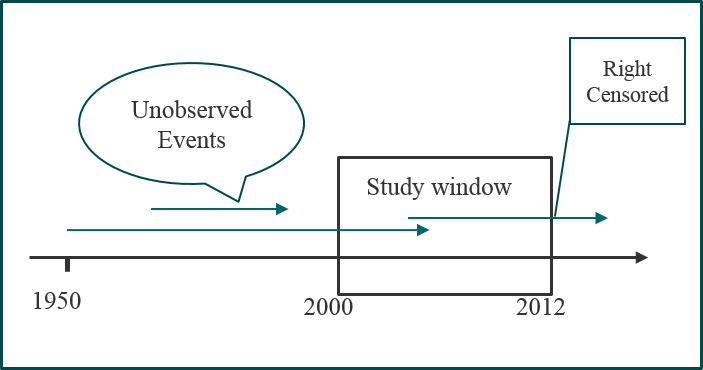
\includegraphics[width=3.5in]{fig1.png}
 	\caption{Right censor and left truncation}
 	\label{fig:1}
 \end{figure}
  Let $T$ denotes the time of main event of interest to occur and let $C$ denotes the end time of study. An observation is right censored when $T> C$, indicating the study do not have the failure time of the right censored observation. In this study, the study window is from November 2000 to December 2012 as shown in the figure \ref{fig:1}. Thus, the current active employees have unknown terminated date. They are treated as right censor. These right censored observations require special treatment in survival analysis: a censor indicator variable is created:
 \begin{align*}
 	\delta_i&=
 	\begin{cases}
 		1   &\text{if  }  t_i \leq c_i \text{ (uncensored),}\\
 		0   &\text{if  }  t_i > c_i \text{ (censored),}
 	\end{cases}
 \end{align*}
 where, $i$ denotes the ith observation, and the failure time of event for ith observation is minimum time between $t_i$ and $c_i$, i.e., $min(t_i, c_i)$, that is when $ c_i <t_i $, $c_i$ is taken as end time of the ith observation in order to do next  analysis.

 Left truncation is that the occurrence of an intermediate event prior to the event of interest appear in the sample dataset. Let $T$ denotes the time of event of interest to occur and let $X$ denotes the time an individual enters the study, that is time of truncation events occurs. Only the individuals with $T \geq X$ are observed in the study window. Left truncation in this study occurs due to no records for employees leaving the organization before November 2000 as unobserved events shown in the figure \ref{fig:1}. The left truncation leads to another bias. As shown in the figure \ref{fig:1}, the longest arrow represents a life span for an employee hired in 1950 and left in 2006. Those employees who remain in the study window increase the apparent lifetimes. The existence of truncation in the data must be taken into account in order to overcome this bias and to achieve accurate estimation of survival analysis \citep{carrion2010}. Let $t_{i0}$ denotes the start time of the ith observation, i.e., hired time or age at hired of ith employee, $x_{i}$ denotes the entry time of the ith observation, i.e., the start time of study (November 1st, 2000) or age at November 1st, 2000. The start time of the observation is maximum value between $t_{i0}$ and $x_i$, that is when $t_{i0} < x_i $, $x_i$ is taken as start time of the ith observation in order to eliminate the left truncation bias \citep{allison1995}. The number of failures in the $t_j$ is redefined for left truncation. When $x_i < t_j \le t_i$, the observation is in the risk set. When $t_{j} < x_i \le t_i$, the ith observation has not entered study yet at $t_j$ and it cannot be considered in the risk set. When $x_i \le t_i < t_j$, it indicates the ith observation whose failure time before $t_j$, and it cannot be considered in the risk set at time $t_j$ neither \citep{carrion2010}.

% simulation study.

\subsection{Cox PH regression model}
%   1. what is cox ph regression model.
Cox proportional hazards (PH) regression is a widely used method for estimating survival life events, introduced in a seminal paper by \citet{cox1972}. The Cox PH model is usually taken the form of hazard model formula as shown in the equation \ref{eq:cox}:
   \begin{equation}
   \label{eq:cox}
   h(t,x)=h_0(t)e^{(\sum_{i=1}^{k}\beta_ix_i)}
   \end{equation}

   where $x=(x_1, x_2, \ldots, x_k)$, $h_0(t)$ is the baseline hazard occurring when $x=0$, $\beta$ is the coefficients of $x$.
%    why not parametric. baseline cannot fit to any parametric model\\
%    2. cox regression without/ with time dependent variable\\
   The model provides a hazard expression at time t for an individual with a given specification of a set of explanatory variables denoted by the $x$. The Cox PH formula is the product of quantities at hazard time $t$: $h_0 (t)$ as the baseline hazard function and the exponential expression to the linear combination of $\beta_i x_i$, $x$ does not involve time $t$, so it is time-independent variables. $x$ can also be time-dependent variables, which named extended Cox PH regression as discussed in the section \ref{sec:coxt}. The key assumption for Cox PH regression model is proportion hazards. However, Cox regression can handle non proportional hazards using time-dependent variable or stratification.
   The Cox PH regression is "robust" and popular, because the baseline hazard function $h_0 (t)$ is an unspecified function and its estimation can closely approximate correct parametric model \citep{kleinbaum1998}. Taking the logarithm of both sides of the equation, the Cox PH model is rewritten in the equation \ref{eq:coxlog}:
   \begin{equation}
   \label{eq:coxlog}
   \log{h(t,x)}=\alpha(t)+\sum_{i=1}^{k}\beta_ix_i
   \end{equation}
   where $\alpha(t)=\log{h_0(t)}$. If $\alpha(t)=\alpha$, the baseline is exponential distribution. In the Cox PH regression, $\alpha(t)$ do not limited on specific parametric distributions and it can take any form. The partial likelihood method is used to estimated $\beta$ coefficients of the Cox model without having to specify the baseline \citep{allison1995}. The Cox PH model is conducted by SAS.


\subsection{Time dependent variable and counting process}
\label{sec:coxt}
A time dependent variable is that a variable is not constant through the whole study and its value changes over the course of the study. The extended Cox PH regression model incorporates both time-independent and time-dependent variables as shown in the equation \ref{eq:timecovar}:
\begin{equation}
\label{eq:timecovar}
h(t,x)=h_0(t)e^{(\sum_{i=1}^{k_1}\beta_ix_i+\sum_{j=1}^{k_2}\gamma_jx_j(t))}
\end{equation}
where $x=(x_1, x_2, \ldots, x_{k_1}, x_1(t), x_2(t), \ldots, x_{k_2}(t))$, $h_0(t)$ is the baseline hazard occurring when $x=0$, $\beta$ and $\gamma$ are the coefficients of $x$.
There are four time dependent variables in this study: {\it policy}, {\it P85}, {\it A65} and economic indicators. Policy is to handle the ERIP issued in January 2008 with three months response time window to accommodate a voluntary reduction in force from the organization.

{\bf citation about ERIP}

Policy is a dummy variable across years:
\begin{align*}
Policy&=
\begin{cases}
1   &\text{if employee works in year 2008,}\\
0   &\text{if  employee does not work in year 2008.}
\end{cases}
\end{align*}

%What is counting process.   \\
Counting process method in SAS programming statements is used to handle time dependent variables, which is each employee have multiple records. Each record is related to a time interval and the variables in this record remain constant.
Therefore, Each employee has up to 3 records: before 2008, in-between 2008, and after 2008 to handle variable policy. Age are used for repenting two time terminals of each interval or record. For age, one time point is age at beginning of the certain period, named "age at start"; and the other one is age at end of the curtain period, named "age at end".

$P85$ and $A65$ are two time dependent dummy variables, representing two retirement requirements for achieving full define benefit: points 85 and age at 65. These two variables also split the three time intervals into two parts: age before reaching point 85 and age after reaching point 85 or age younger than 65 and age equal or older than 65. 
 
Economic indicators is another time dependent variables. Because economic indicators are fluctuated across the year, all the employees have up to 12 years records based on the calender year, which interval starts from hired date or January 1, and ends at terminated date or December 31 of certain year during the study window as shown in equation \ref{eq:interval}. The economic indicators are taken the average value for each year into the optimal model identified from the internal variables to examine their impacts on turnover.
\begin{equation}
\label{eq:interval}
\begin{split}
(\text{start point}, \text{end point})= (max(\text{hired date}, \text{January 1 of a certain year}),\\
min(\text{terminated date}, \text{December 31 of a certain year}))
\end{split}
\end{equation}


\subsection{Stratification model}
%I. what is stratification model;\\
An alternative for handling nonproportional hazards is stratification.  A stratified model allows each subgroup of data as defined by a grouping variable to have its own baseline hazard while sharing parameters for other variables across. If the proportional hazards assumption holds within these subgroups then this model allows us to get valid common estimates of variable effects using all of the observations. Equation \ref{eq:strata} below represents the hazard function for strata {\it z};
\begin{equation}
	\label{eq:strata}
	h(t,x,z)=h^z_0(t)e^{(\sum_{i=1}^{k}\beta_ix_i)}
\end{equation}
where $z$ represents the grouping variable, and $h^z\sigma_0(t)$ is a baseline hazard based for stratam z and $\beta_i$ are common effects of variables ac. Note that the strata variables cannot be the variables in the Cox PH model.

%II. how to select a stratify variable\\
The proportional hazard assumption can be tested using Schoenfeld residuals which works even if the model includes time-dependent variables; see \citet{allison2010,collett2015}. An alternative is to test the interaction between time-dependent and time-independent variables in the Cox PH model. The assumption is valid if the interaction is not statistically significant ($P>0.05$).  Including a stratified variable, when appropriate, can improve the Cox model's performance.  The C-statistic is used to compare models with and without stratification with a higher C value indicating a better model \citep{lemke2012}.

\subsection{Competing risks}
%  what is competing risks. competing ricks can help forecasting employee retirement and voluntary quit. \\
%  why select these two reasons to model.\\
  A competing risk is an event whose occurrence either precludes the occurrence of the event of interest or fundamentally alters the probability of occurrence of this event of interest \citep{tableman2003}. For example, turnover causes of an employee are exclusive and independent, i.e. an employee can experience only one event such as voluntary quit rather than retirement. This alters the probability of experiencing the event of interest, like retirement. Such events are known as competing risks events where one event of several different types of possible events can occur and hence the survival analysis for each event is calculated separately with the other events set as censored. Two mutually exclusive causes: retirement and voluntary quit are considered as the event of interests for each employees in this study, and the other events are treat as censored.

  There are several reasons for selecting retirement. One main reason is because the organization are interested in forecasting the turnover of retirement. There are $1/3$  employees in that organization are over 50 years old who are eligible for retirement. And, some other reasons of turnover, such as layoff, transfer, death, or disability are caused by the factors which occurrence are random and hard to predict. The Cox PH regression for competing risks as shown in equation \ref{eq:competing}:
  \begin{equation}
  \label{eq:competing}
  h_j(t,x)=h_{j0}(t)e^{(\sum_{i=1}^{k}\beta_{ij}x_i)}
  \end{equation}
  where, $x_{j}$ is the variable for a specific type of turnover. Note that the coefficient $\beta$ is the effects of the variables may be different from different turnover types. If $\beta_{ij}$  is the same for all j, the model simplified to Cox PH model as shown in equation \ref{eq:cox}.


\subsection{Variable selection}
All the variables are putting into Cox PH regression model and selected by manually backwards selection method based on $P<0.05$.  The variable selection procedure is as follow: first, all the variables are used to build the model. Second, remove the non-significant variable ($P>0.05$) with the largest P value, and rerun the model with the other variables. Then, repeat the second step until there is no significant variable remaining in the model.
\subsection{Model evaluation and comparison}
%\subsubsection{Measurements}
%AIC, BIC, MAPE, c statistic.\\

The Cox PH model is evaluated by four statistics criteria:  Akaike’s information (AIC), Schwartz’s Bayesian criterion (SBC), mean absolute percentage value (MAPE) and $G^2$. The optimal model should have low AIC, SBC, MAPE, and $G^2$ value for both training and holdout dataset. In this study, the model performance on holdout dataset is considered more important than that on the training dataset.  AIC and SBC are both information criteria using likelihood value. Usually, the best model comes with lowest AIC or SBC values. AIC, SBC values are automatically generated by the models.

%C-statistics or the area under the receiver operating characteristic (ROC) curve is to test whether the probability of predicting the outcome is better than chance. It ranges from 0.5 to 1.  Models are considered acceptable when the C-statistic is higher than 0.7 \citep{hosmer2013}. C-statistics are calculated by using the predicted failure probability compared with the actual outcomes by SAS proc logistic. 
The predicted failure (retirement) probability is actually the conditional failure probability for an employee at time $t_j$, given that the employee is active at time $t_{j-1}$. It is calculated based on the baseline and coefficients from Cox PH models for both training and holdout dataset as shown in equation \ref{eq:prob}.
\begin{equation}
\label{eq:prob}
\begin{split}% to allgin the equation
P\{t_{j-1}<T<t_j\} &=1-P\{T>t_j|T \ge t_j\}\\
&=1-\frac{S_{t_j}}{S_{t_{j-1}}}   \\
&=1-\frac{{S_0(t_j)}^{(\sum_{i=1}^{k}\beta_ix_i)}}{   {S_0(t_{j-1})}^{(\sum_{i=1}^{k}\beta_ix_i)}}
\end{split}
\end{equation}
where, $T$ is survival time, $t_j$ is a specific value for $T$, $S_0(t)$ is the baseline function generated by Cox PH model, $x$ is the variables, and $\beta$ is the coefficient.

MAPE is another measure for comparing the accuracy of the model fitting between different forecast models since it measures relative performance \citep{chu1998} as shown in the equation \ref{eq:mape}.
\begin{equation}
	\label{eq:mape}
	MAPE=\sum_{t=1}^{n}\left | \frac{y_t-\hat{y_t}}{y_t} \right |\frac{1}{n}\%
\end{equation}
MAPE is calculated by using the yearly actual and predicted retirement number as $y_t$ and $\hat{y_t}$, respectively.
The predicted retirement or voluntary quit number is the expected retirement or voluntary number summarized by aggregating all the failure probabilities for the active employees in the risk set at $t_j$ as shown in \ref{eq:expturnover}.
\begin{equation}
\label{eq:expturnover}
E(\text{turnover number at } t_j)=\sum_{i=1}^k{P_i\{t_{j-1}<T<t_j\}}
\end{equation}
where, $i$ denotes the ith employee.

$G^2$ is another criteria to evaluate the model prediction performance. The calculation takes the form as shown in the equation \ref{eq:g2} \citep{simonoff2013},
\begin{equation}
\label{eq:g2}
G^2=2\sum_{t}[y_t\log{(\frac{\bar{p_t}}{\hat{p_t}}})+ (n_t-y_t)\log{(\frac{1-\bar{p_t}}{1-\hat{p_t}}})]
\end{equation}
where, $y_t$ is the number of employees retired in year $t$, $n_t$ is the workforce number in year $t$, $\bar{p_t}={y_t}/{n_t}$, and $\hat{p_t}={\hat{y_t}}/{n_t} $.


%%%%%%% need some explain for traing and holdout mape%%%%%%%%%%%
The logistic regression and time series moving average methods are also employed to compare with the  performance of Cox PH regression model by MAPE value and $G^2$.
%The evaluation step is to calculate the yearly predicted turnover number for training and holdout dataset, and then compared the predicted number with the actual number.


%add evaluation formula.

%\subsubsection{Model validation}
% 1. Forecast employee turnover   how to forecast and calculate employee turnover number\\
% 2. conditional probability (The prediction is conditional probability): given the employee is survival at last year, what is the probability they survival or quit for this year.\\
% 3. the total number of employee turnover is the aggregate all turnover probabilities of employees at each year\\
%
% 4. split data into two ways: both training and holdout, training to build the model and holdout is to validate the model, and compare the actual vs forecasting, calculated MAPE and C statistics. \\
%       WAY1: training (10 years)and holdout (2 years). forecasting the total number of employee leaving the organization, compared to the actual number to calculate MAPE and C statistics. compare to logistic regression and time series methods to shown survival is better.\\
%       WAY2: random split the data into training (2/3) and holdout (1/3), using c statistics to select one best survival model.
 \subsection{Simulation on right censor and left truncation}

 In order to understand the performance and efficiency of the Cox PH model in right censored and left truncated data we perform a simulation study.

 Generated $n =100, 200, 500, 1000, 2000, \text{and } 4000$ observations  from a Weibull regression model  with one variable which we referred to as age.

 Age is uniformly distributed from 22 to 70 years of age, which is chosen to mimic the actual distribution of workers ages in our sample.

 In the regression model, the coefficients for $\beta_{age} = -.025$ (Why?) and the coefficient for $\beta_0 = 1.5$.

 The survival times $T_i$ are randomly generated from a Weibull distribution with shape parameter $\alpha$ and scale parameter $\lambda$, where $\alpha=1.5$ and $\lambda=exp(-0.025age+\beta_0)^{\frac{1}{\alpha}}$.


% The simulation is used to examine Cox PH model predictive performance with right censor and left truncation. The simulated lifetime data is generated based on the Weibull distribution. %The hazarld function for Weibull regression model with shape parameter $\alpha$, scale parameter $\lambda$, and variable $X$ is shown in equation \ref{eq:weibul}, given $h_0=\alpha(\lambda)^\alpha t^{\alpha-1}$:
 %\begin{equation} \label{eq:weibul}
 %\begin{split}% to allgin the equation
 %h(t|X) & =h_0(t)exp(\beta X) \\
 %         &=\alpha (\lambda (exp(\beta X)^{\frac{1}{\alpha}})^\alpha t^{\alpha-1} \\
 %         &=\alpha(\tilde{\lambda} )^\alpha t^{\alpha-1}
 %\end{split}
 %\end{equation}
 %where, $\tilde{\lambda}=\lambda (exp(\beta X)^{\frac{1}{\alpha}}$.
% The simulation can be described as follows. The sample size was n=100, 300, 500, 1000, and 4000, with one variable $X$, named Age, which follows uniform distribution with parameter $a$ $(a=22)$ and $b$ $(b=70)$. Only one variable age is used in simulation process to make the estimation procedure simple and close to real world. The coefficient $\beta_{age}$ is taken $-0.025$ and $\beta_0=1.5$.
%Then, the survival time $T$ is random generated for each observation based on Weibull distribution with shape parameter $\alpha$ and scale parameter $\lambda$, where $\alpha=1.5$ and $\lambda=exp(-0.025age+\beta_0)^{\frac{1}{\alpha}}$.

 The simulation is performed on right censoring and left truncation separately, in order to observe the effects for different bias.
 For right censor simulation, two simulation procedure are conducted with different start points. First, the start point for all the observations are equal to 0, and stop point is equal to the survival time $t_i$ for ith observation where $T=(t_1, t_2, \ldots, t_n)$. After that, the censor time $C$ is equal to first quarter, median, third quarter, and maximum of the survival time, respectively, to get 75\%, 50\%, 25\% and 0\% censor proportions. When the survival time $t_i$ for ith observation is not greater than the censor time ($c_i$), the stop point is survival time $t_i$ and censor variable $\delta_i$ is 1. When survival time $t_i$ for ith observation is greater than censor time ($c_i$), the stop point is change to censor time ($c_i$) and censor variable $\delta_i$ is 0. The second right censor simulation procedure is to set the start points $S$ to follow uniform distribution from 0 to 10, representing the observations (employees) start at various time points within 10 years study window. The stop point is equal to the summation of start point and survival time: $S+T$. The censor time is a cutoff point ($C$) identified by R to get fix number of censor proportion (25\%, 50\%, and 75\%).  When the survival time $t_i$ for ith observation is not greater than the censor time ($c_i$), the stop point is survival time $t_i$ and censor variable $\delta_i$ is 1. The stop points are set to censor time $C$ for the observations with the stop points $S+T$ being great than censor time $C$, the survival time is reset to $C-S$, and censor variable $\delta_i$ is 0. Otherwise, the other observations with stop point being less than the censor time remain the same and the censor variable $\delta_i$ is 1. For the second simulation, there are 4000 observations are generated. Because some observations occur after the cutoff point (censor time) and the sample size are various for different censor proportion, only 400 are randomly selected with 75\%, 50\%, 25\% and 0\% censor proportions to keep the sample size same. The start point and the stop point are dependent variable in the cox regression model. $\delta$ is censor variable.

 For left truncation simulation, the start point $U$ is generated as uniform distribution with $a=0$ and $b=max(T)$ which indicates an observation start randomly from time 0 to time $max(T)$. The stop point $S$ is $U+T$. The histogram is generated for $S$. The truncation time $L$ is set as 0, first quarter, median, and third quarter of $S$, respectively, to get 0\%, 25\%, 50\%, and 75\% truncation proportions. When start point $u_i$ for ith observation is less than truncation time $l_i$, the start point is reset as truncation time $l_i$. When start point $u_i$ for ith observation is not less than truncation time $l_i$, the start point does not change ($u_i$). In left truncation, the censor variable $\delta$ for all the observations are equal 1. For right censor and left truncation simulation,  the Cox regression models are modeled by "coxreg" and "phreg" function in eha package. The coxreg function is the regular cox regression modeling procedure to generate coefficient estimates and a non-parametric baseline.  The phreg funcation is using parametric distribution like Weibull, Extrem value (EV) to estimate the baseline. The "phreg" function performs Cox PH model and also provides a parametric baseline hazards estimation \citep{brostrom2012}. The phreg function is used to compare the non-parametric with parametric baseline and to demonstrate the prediction when the parametric baseline is not right.
 Total predicted failure number is calculated as shown in equation \ref{eq:prob} and \ref {eq:expturnover}. The actual and predicted failure number are compared to show right censor and left truncation's impacts on the coefficient and baseline estimation .

 %accelarate model%
\section{Results}
\subsection{Right censor and left truncation simulation results}
% 1. right censor start 0 results shows in table 1a
% 2. start different results shows in table 2 and figure 2 with different baseline and prediction number
%    younger company has shorter baseline hard to predict beyond the baseline max time.
% 3. left truncation simulation results shows in table 1 and figure 4&5
% 4. shows the baseline using wrong parametric distribution (wrong) what is going on.
The right censoring simulation results are shown in the left part of Table \ref{tab:rightcensor} which all the observations start at the same time 0. The events in the second column of the table are the actual total failure events simulated without considering censoring, which is $n=100, 200, 500, 1000, 2000, \text{and } 4000$. The number of events in the dataset applying to the Cox model are reduced due to the right censoring, which is equal to $events=\sum_{i=0}^{n}{\delta_i}$. The values in the other column are the average value of 100 replications for Cox PH model coefficient and baseline parameter estimates based on Weibull distribution using phreg. The simulation results show censoring proportion and the number of events are two influential factors for the coefficient estimation. The model overestimates the coefficients of age, $\lambda, \text{ and } \alpha$, when the dataset has high proportion of censoring. For example, when 75\% of the data are censored with only 25 events, the estimates for three parameters are 0.028, 4.043, and 1.564, respectively, which are the highest among all the estimates. As the event number increasing, the estimation is approaching to the actual value. For example, the estimation of age, $\lambda, \text{ and } \alpha$ are close to 0.025, 2.7, and 1.5, respectively, after the number of event is at least 500.
The predicted events in the sixth column is the total predicted failure number calculated by applying the coefficient estimates and the non-parametric baseline from Cox PH models into the dataset without considering censoring. The predicted events using censoring models are all lower than the actual total failure number, but close to the number of events after censoring. For example, the number of predicted events is 24.84 when using the estimates of Cox PH model with 75\% censoring to calculate the dataset with 100 events, which is close to 25. The prediction is less than the actual dataset, because the baseline is lack of information for the events after censored time. The baseline does not include hazards or survival probability information for the long life time observation, because the baseline just captures the events before the censor time and the observation with long life time are censored in this simulation. As a result, there is no failure probability for long life time observation.

\begin{table}[htbp]
	\renewcommand{\arraystretch}{1.5}
	\scriptsize %table fond
	\centering
	\caption{Right censoring and left truncation simulation statistics}
	
	\begin{tabular}{cccccc||cccccc}
		\hline
		\multicolumn{1}{c}{\multirow{2}{1.5cm}{Censor proportion}} & \multicolumn{1}{c}{\multirow{2}[3]{*}{Events}} & \multicolumn{3}{c}{Variable Estimates} & \multicolumn{1}{c}{\multirow{2}{1cm}{Predicted Events}} & \multicolumn{1}{c}{\multirow{2}{1.5cm}{Truncation proportion}} & \multicolumn{1}{c}{\multirow{2}[3]{*}{Events}} & \multicolumn{3}{c}{Variable Estimates} & \multicolumn{1}{c}{\multirow{2}{1cm}{Predicted Events}} \\
		\cline{3-5}
	    \cline{9-11}
		\multicolumn{1}{c}{} & \multicolumn{1}{c}{} & Age   & $\lambda$ & $\alpha$ & \multicolumn{1}{c}{} & \multicolumn{1}{c}{} & \multicolumn{1}{c}{} & Age   & $\lambda$ & $\alpha$ & \multicolumn{1}{c}{} \\
		\hline
				0\%   & 100   & 0.026 & 2.931 & 1.509 & 97.42 & 0\%   & 100 & 0.027 & 2.865 & 1.534 & 96.60 \\
				25\%  & 100    & 0.027 & 2.962 & 1.527 & 74.31 & 25\%  & 75 & 0.027 & 2.917 & 1.546 & 72.86 \\
				50\%  & 100    & 0.028 & 3.237 & 1.530 & 49.66 & 50\%  & 50 & 0.027 & 2.899 & 1.577 & 47.32 \\
				75\%  & 100    & 0.028 & 4.043 & 1.564 & 24.84 & 75\%  & 25 & 0.029 & 3.280 & 1.757 & 21.75 \\
				0\%   & 200   & 0.026 & 2.841 & 1.508 & 197.23 & 0\%   & 200 & 0.025 & 2.777 & 1.506 & 196.13 \\
				25\%  & 200   & 0.026 & 2.856 & 1.513 & 149.34 & 25\%  & 150   & 0.025 & 2.756 & 1.515 & 147.97 \\
				50\%  & 200   & 0.026 & 2.925 & 1.527 & 99.68 & 50\%  & 100   & 0.025 & 2.825 & 1.532 & 97.44 \\
				75\%  & 200    & 0.026 & 3.167 & 1.540 & 49.86 & 75\%  & 50    & 0.026 & 2.927 & 1.572 & 47.17 \\
				0\%   & 500   & 0.025 & 2.731 & 1.500 & 496.77 & 0\%   & 500 & 0.025 & 2.732 & 1.509 & 494.78 \\
				25\%  & 500   & 0.025 & 2.718 & 1.508 & 374.31 & 25\%  & 375 & 0.025 & 2.737 & 1.514 & 373.42 \\
				50\%  & 500   & 0.025 & 2.744 & 1.514 & 249.65 & 50\%  & 250 & 0.026 & 2.778 & 1.514 & 247.70 \\
				75\%  & 500   & 0.025 & 2.787 & 1.525 & 124.89 & 75\%  & 125 & 0.026 & 2.835 & 1.547 & 124.15 \\
				0\%   & 1000  & 0.025 & 2.748 & 1.509 & 996.41 & 0\%   & 1000 & 0.025 & 2.710 & 1.504 & 993.77 \\
				25\%  & 1000   & 0.025 & 2.747 & 1.512 & 749.23 & 25\%  & 750 & 0.025 & 2.709 & 1.504 & 748.94 \\
				50\%  & 1000   & 0.025 & 2.748 & 1.514 & 499.61 & 50\%  & 500 & 0.025 & 2.715 & 1.506 & 503.37 \\
				75\%  & 1000   & 0.026 & 2.844 & 1.509 & 249.80 & 75\%  & 250 & 0.025 & 2.694 & 1.524 & 250.93 \\
				0\%   & 2000  & 0.025 & 2.714 & 1.502 & 1996.19 & 0\%   & 2000 & 0.025 & 2.740 & 1.503 & 1993.65 \\
				25\%  & 2000  & 0.025 & 2.713 & 1.503 & 1499.29 & 25\%  & 1500 & 0.025 & 2.731 & 1.502 & 1507.94 \\
				50\%  & 2000  & 0.025 & 2.742 & 1.500 & 999.68 & 50\%  & 1000  & 0.025 & 2.724 & 1.503 & 1012.37 \\
				75\%  & 2000   & 0.025 & 2.733 & 1.502 & 499.89 & 75\%  & 500 & 0.025 & 2.718 & 1.508 & 512.30 \\
				0\%   & 4000  & 0.025 & 2.719 & 1.504 & 3995.80 & 0\%   & 4000 & 0.025 & 2.720 & 1.500 & 3988.90 \\
				25\%  & 4000  & 0.025 & 2.718 & 1.505 & 2998.86 & 25\%  & 3000 & 0.025 & 2.722 & 1.501 & 3014.31 \\
				50\%  & 4000  & 0.025 & 2.724 & 1.503 & 1999.52 & 50\%  & 2000 & 0.025 & 2.710 & 1.502 & 2032.03 \\
				75\%  & 4000  & 0.025 & 2.729 & 1.513 & 999.86 & 75\%  & 1000 & 0.025 & 2.703 & 1.503 & 1028.39 \\
				\bottomrule
	\end{tabular}%
	\label{tab:rightcensor}%
\end{table}%

% Table generated by Excel2LaTeX from sheet 'Sheet2'
\begin{table}[htbp]
	\renewcommand{\arraystretch}{1.5}
	%\scriptsize %table fond
	\centering
	\caption{Right censor simulation results by various start time}
	\begin{tabular}{ccccccc}
		\toprule
    	\multicolumn{1}{c}{\multirow{2}{1.5cm}{Censor proportion}}  & \multirow{2}[4]{*}{Events} & \multicolumn{3}{c}{Variable Estimaties} & \multicolumn{2}{c}{Predicted Events} \\ \cline{3-7}
		     &       & Age   & $\lambda$ & $\alpha$ & "coxreg" & "phreg" \\
		\midrule
		0\%   & 400   & 0.025 & 2.694 & 1.508 & 398.52 & 400.44 \\
		25\%  & 400   & 0.026 & 2.802 & 1.518 & 394.24 & 401.72 \\
		50\%  & 400   & 0.026 & 2.828 & 1.514 & 340.73 & 398.51 \\
		75\%  & 400   & 0.025 & 2.821 & 1.518 & 215.92 & 400.80 \\
		\bottomrule
	\end{tabular}%
	\label{tab:right2}%
\end{table}%


\begin{figure}[h!]
	\centering
	\subfloat[No right censor ]{\label{fig:baseno}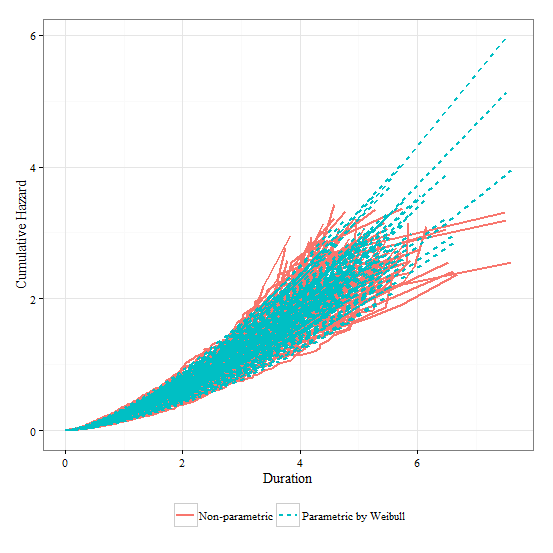
\includegraphics[width=3in]{base0.png}}
	\quad
	\subfloat[25\% right censor]{\label{fig:base25}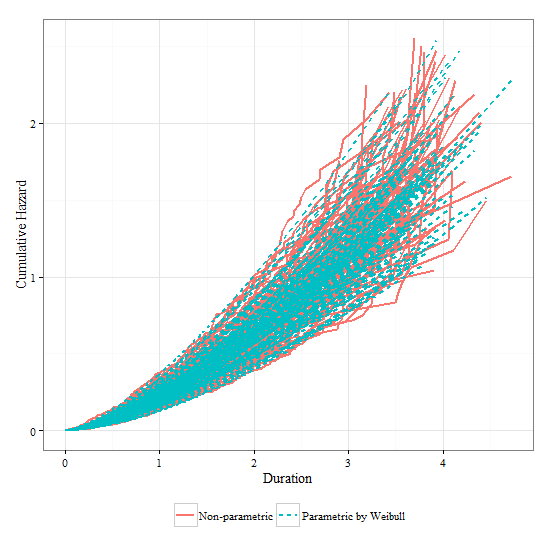
\includegraphics[width=3in]{base25.png}}
	\quad
	\subfloat[50\% right censor ]{\label{fig:base50}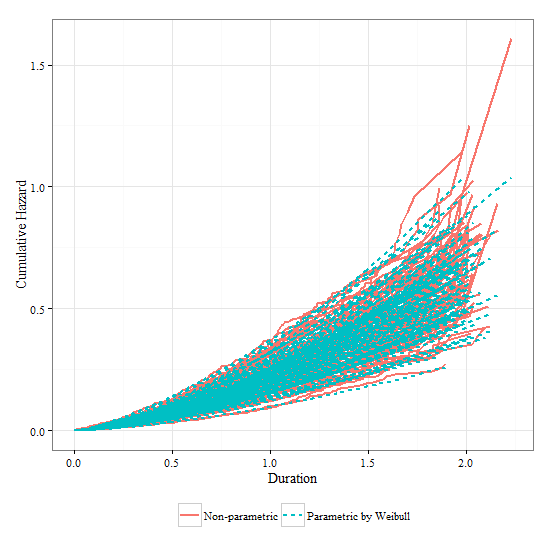
\includegraphics[width=3in]{base50.png}}
	\quad
	\subfloat[75\% right censor]{\label{fig:base75}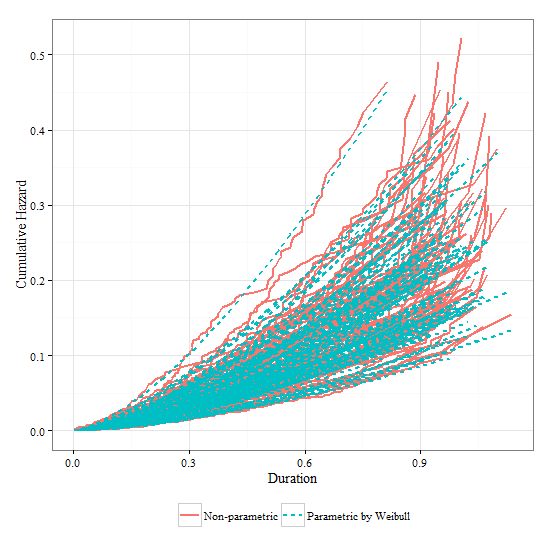
\includegraphics[width=3in]{base75.png}}
	\caption{Baseline comparison by various censoring}
	\label{fig:rightbase}
\end{figure}

\begin{figure}[h!]
	\centering
	\subfloat[No right censor ]{\label{fig:rightno}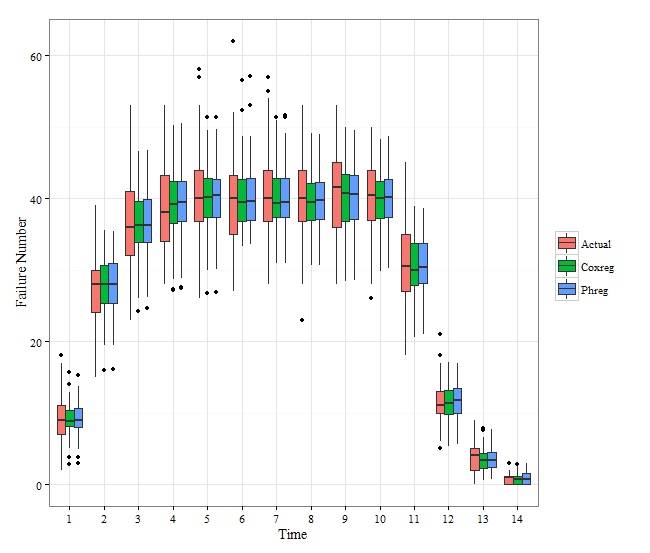
\includegraphics[width=3in]{right0.png}}
	\quad
	\subfloat[25\% right censor]{\label{fig:right25}\includegraphics[width=3in]{right25.png}}
	\quad
	\subfloat[50\% right censor ]{\label{fig:right50}\includegraphics[width=3in]{right50.png}}
	\quad
	\subfloat[75\% right censor]{\label{fig:right75}\includegraphics[width=3in]{right75.png}}
	\caption{Right censor simulation results: actual vs. predicted failure number}
	\label{fig:rightpred}
\end{figure}

To simulate the realistic situation, the second right censor simulation is conducted with randomly occurrence of the observations followed by uniform distribution. The results are shown in the table \ref{tab:right2}. The events without considering censoring are all equal to 400 for easy comparison. The predicted events include the prediction by non-parametric baselines using "coxreg" and by parametric baseline using "phreg" function Weibull distribution as baseline estimation. The estimation of age and $\alpha$ are all close to the simulated value (0.025 and 1.5). And the estimation of $\lambda$ are around 2.8. These indicate the right censoring does not impact the coefficients estimation. However, right censoring does impact the baseline function estimation for Cox PH model as shown in the figure \ref{fig:rightbase}. The red lines in the figure \ref{fig:rightbase} are the non-parametric baseline for 100 replications. And blue dash lines are the parametric baseline generated base on Weibull distribution for 100 replications, which represent the actual baseline. All these baselines are overlap together by various censoring, which indicates non-parametric baseline can capture the true parametric baseline. However, the duration of the non-parametric baseline is getting short by increasing the censoring proportion. As a result, the predicted number of events using non-parametric baseline is less than the actual failure number. However, it does not affect the prediction by using parametric baseline, which are all close to 400, because the parametric baseline is not limited by the baseline duration if the parameters are correctly estimated. The prediction by "coxreg" and "phreg" are plotted across time by box plot to compare to the actual failure values as shown in the figure \ref{fig:rightpred}. The vertical red line is the average value of censor time. The predicted number of events by "coxreg" are close to actual and the prediction by "phreg" before the censor time line. It is still close to actual after censor time line for the data with no censoring and with 25\% of censoring as shown in the figure \ref{fig:rightno} and \ref{fig:right25}, because of the long baseline duration. However, It drops down gradually after the censor time for the data with 50\% and 75\% of censoring as shown in figure \ref{fig:right50} and \ref{fig:right75}, because the baseline duration ends around censor time. This simulation clearly shows the limitation of Cox PH model with
non-parametric baseline: it cannot accurate predict far beyond the duration of the longest events. Therefore, a baseline can be highly variable in the extremes leading to poor predictions. Although this simulates the real problem, the employee hiring time points are followed by uniform distribution in the real world.

% % % % % % % % % % % % % % % % % % % % % % % % %
% % % %Left truncation result % % % % % % % % % %
% % % % % % % % % % % % % % % % % % % % % % % % %
\begin{figure}[h!]
	\centering
	\subfloat[No left truncation]{\label{fig:ev0}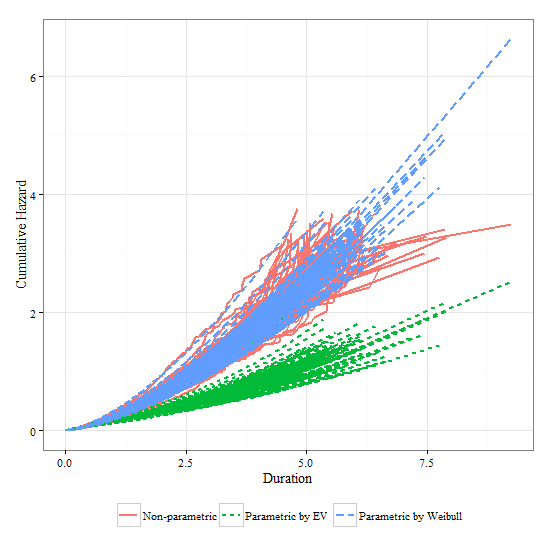
\includegraphics[width=3in]{EV0.png}}
	\quad
	\subfloat[25\% left truncation]{\label{fig:ev25}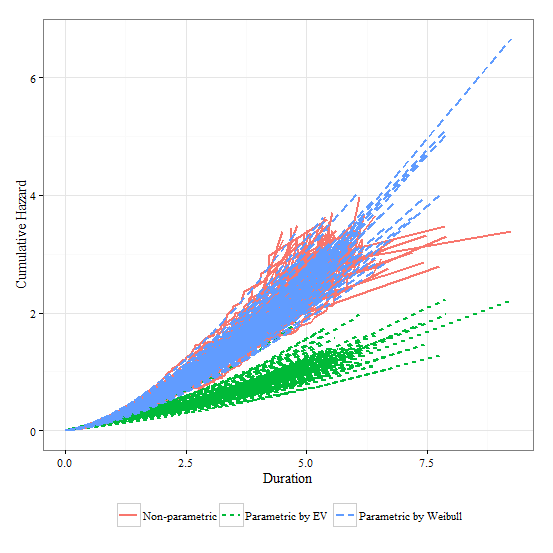
\includegraphics[width=3in]{EV25.png}}
	\quad
	\subfloat[50\% left truncation]{\label{fig:ev50}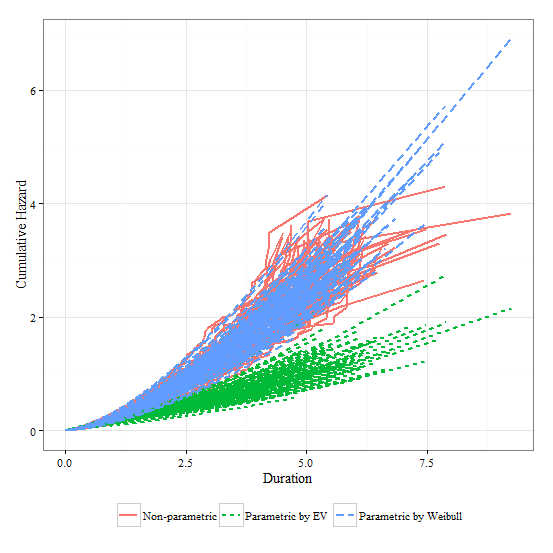
\includegraphics[width=3in]{EV50.png}}
	\quad
	\subfloat[75\% left truncation]{\label{fig:ev75}\includegraphics[width=3in]{EV75.png}}
	\caption{Left truncation simulation results: Baseline Comparison}
	\label{fig:leftbase}
\end{figure}

\begin{figure}[h!]
	\centering
	\subfloat[No left truncation]{\label{fig:leftno}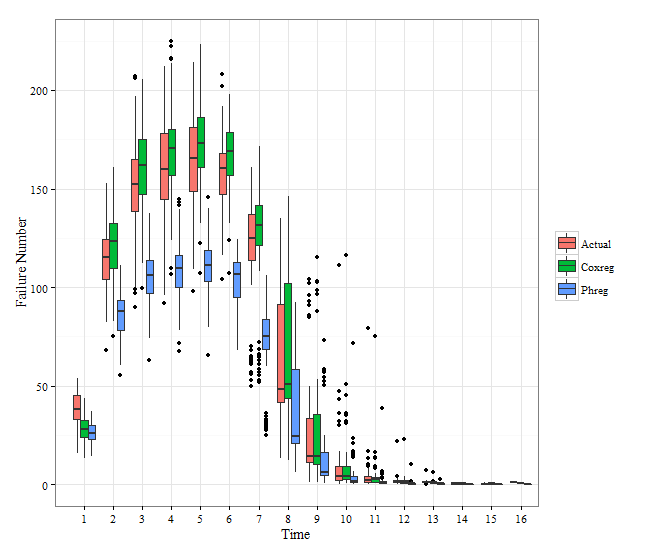
\includegraphics[width=3in]{Predev0.png}}
	\quad
	\subfloat[25\% left truncation]{\label{fig:left25}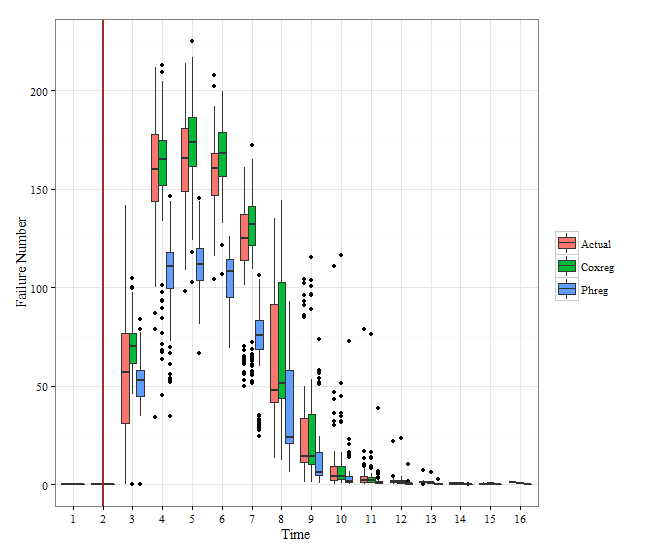
\includegraphics[width=3in]{Predev25.png}}
	\quad
	\subfloat[50\% left truncation]{\label{fig:left50}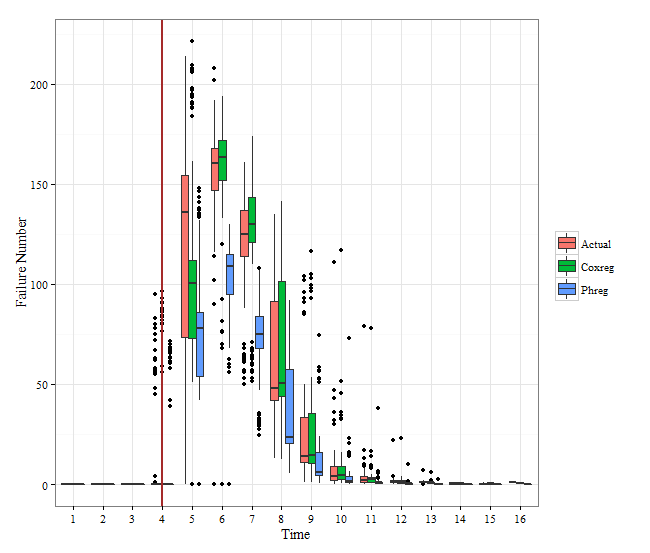
\includegraphics[width=3in]{Predev50.png}}
	\quad
	\subfloat[75\% left truncation]{\label{fig:left75}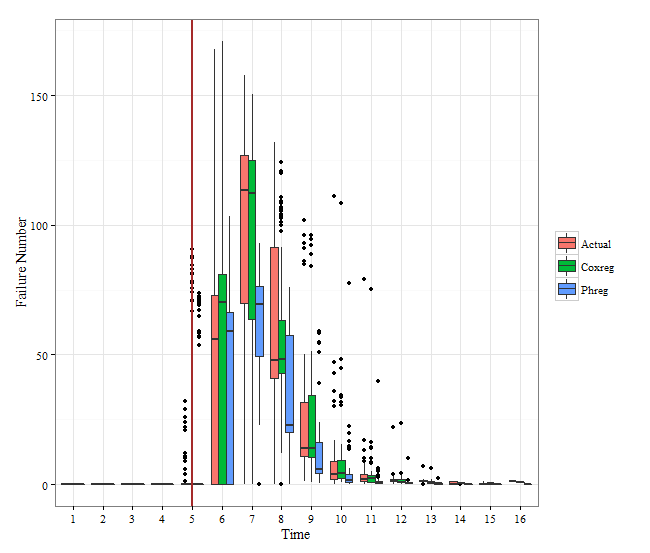
\includegraphics[width=3in]{Predev75.png}}
	\caption{Left truncation simulation results: actual vs. predicted failure number}
	\label{fig:lefttruncation}
\end{figure}
The results of the left truncation bias simulation statistics are shown in the right part of table \ref{tab:rightcensor}. All the values shown are the average value for coefficient estimate of age, and baseline parameter estimates of $\lambda$ and $\alpha$ by "phreg" Weibull distribution. The last column is the total predicted number of events using non-parametric baseline by "coxreg" function. Similar as the right censor simulation result, left truncation proportion and the number of events are two key factors for coefficients estimation. As table \ref{tab:rightcensor} shown, the coefficients are overestimated when the left truncation proportion is 75\% or the number of events are less than 200. However, increasing the number of events can offset (reduce) the left truncation effects. For example, the estimates for age and $\alpha$ are all close to simulated value, when the number of events is 1000 with 75\% truncation proportion. The predicted number of events is close to the actual one as shown the green and red box in the figure \ref{fig:lefttruncation}, which is the box plot of total 2000 events simulated with 100 replication by various proportion of left truncation. The red vertical line is the average of left truncation time. It is slightly overestimated using "coxreg" non-parametric baseline by four left truncation proportions, because the baseline estimation is not affected by the left truncation. The figure \ref{fig:leftbase} clear shows the duration of non-parametric baseline are the same for four left truncation proportion. It also shows the non-parametric baselines (red lines) are overlap with parametric baseline (blue dash lines).

To further test how baseline estimation impacts on the prediction, another simulation is conducted accompanied with left truncation simulation. In the previous left truncations study, the parametric baseline using Extreme Value (EV) distribution is generated by "phreg" and predicted the number of events based on it shape and scale parameter estimation as shown in figure \ref{fig:leftbase}. Because the data is generated by Weibull distribution, the parametric baselines (green dash line) by EV are much lower than the other two baselines by all four left truncation proportions. The predicted number of events based on the EV baseline are also much lower than the actual number of events across the time as the blue box shown in the figure \ref{fig:lefttruncation}. This study shows the inaccuracy estimation of the baseline lead to poor prediction.

Therefore, accurate estimation of coefficients and the baseline are two key factors impacts the perdition of the events of the Cox PH model. The simulation test shows that the Cox PH model can accurately estimates the coefficients when events number is at least 1000 even with high proportion of censor and left truncation. The baseline is another key factor to predict the number of events. The prediction will be accurate if the parametric distribution of the baseline is known or identify the correctly. Otherwise, a wrong baseline can also deteriorate the prediction. Compared to parametric baselines, a non-parametric baseline is more robust. However, it still needs enough number of events with curtain long period to get a smoothed and long baseline to predict accurately. As a result, it is hard to accurately predict the employee turnover for a company just formed recently, or when the employee population characteristic changed, due to high proportion of censor and lack of events. Although this study has more than 50\% right censor, it still has more than 3000 events with long duration (around 50 years length).






% 1- include the name of the package in the Results sections.
% 2 - redo with results averaged over 100 data sets.
% 3 - explain concerns about censoring in our data.  About 50 % censored.  Large amount of truncation.
% 4) - Baseline can be highly variable in the extremes leading to poor
% 5) Figures and discussion of coefficients and baseline estimates and impact on predictions.
% 6) Problems with PH in predictive modelling.  Truncation needs PH (is there another method)
%

% Table generated by Excel2LaTeX from sheet 'Sheet6'



\subsection{Data pattern/Descriptive Analysis}

The construction of a predictive model for retirement involves consideration of several factors. Among the variables available for analysis we must choose the set that offers the maximum predictive power, i.e. a model that includes variables that provide the best possible predictions on out of sample testing data sets and not simply on data used to train the model.  We must also evaluate potential strengths and weaknesses of the baseline hazard estimate and its impact on prediction accuracy.  Finally, it is useful to also understand the impact of various predictors on retirement age.

As described in Section \ref{data.desc}, the current data provides five demographic and career history variables: payroll(hourly, weekly, or monthly payroll), gender(M,F), division(ten divisions), occupational codes(crafts, engineers, general administrative, laborers, managers, administrative, operators, scientists, technicians), age at hire, and years of service at hire. Table \ref{tab:descriptive} provides marginal counts of the number of workers in the sample within each category.  From that we see that among occupation codes there are four large categories (C,E,M,\& P)  with over one thousand employees observed throughout the data sample, four medium sized groups with 500-700 employees (G,L,R \& T), and one small group, S, with 208 employees.  Payroll data shows that the largest group is paid monthly, followed by hourly, and weekly.  In terms of gender, approximately 72\% of employees are male. Finally, divisions, while not fixed over the life of the employee, are distributed similarly to occupational codes with four larger groups and a number of smaller groups.

Beyond these demographic and career factors, our models also include behavioral variables derived from policy requirements for retirement and early retirement incentives that occur throughout the observation period. Histograms of retirement age and accumulated pension points are shown in Figure \ref{fig:hist}. The histogram of for age at retirement is right skewed and shows an anomalous spike at age equals 62 which is the mode, because age 62 is the earliest age for a person to receive social security retirement benefit.
% 79\% of the employees retired at 62 also reach or exceed 85 points. (Why is this such a popular age?  Medicare, Social Security?)  
The average age is 59.72 demonstrating that many individuals retire before 62 and most before age 70. In terms of points accrued at time of retirement, recall that points are the sum of years of service plus current age, we see an irregular distribution with the vast majority retiring with point totals in the range of 85 to 100 and relatively few taking a reduced pension are retiring with diminished benefits with points below 85. Again we see that 85 points is the mode indicating that retiring immediately after become fully vested in the pension is a popular choice.


\begin{table}[htbp]
	\centering
	\scriptsize
		\renewcommand{\arraystretch}{1.5}
	\caption{Descriptive Statistics}
	\begin{tabular}{lrrlrr}
		\toprule
	\textbf{Variable}	& \multicolumn{1}{c}{\textbf{Count}} & \multicolumn{1}{c}{\textbf{N \%}}  &   \textbf{Variable}    & \multicolumn{1}{c}{\textbf{Count}} & \multicolumn{1}{c}{\textbf{N \%}} \\
		\midrule
		\textbf{Cocscode} &       &       & \textbf{Gender} &       &  \\
		C     & 1295  & 16.0\% & F     & 2296  & 28.4\% \\
		E     & 1361  & 16.8\% & M     & 5802  & 71.6\% \\
		G     & 574   & 7.1\% & \textbf{Division} &       &  \\
		L     & 613   & 7.6\% & divison1 & 1542  & 19.0\% \\
		M     & 1178  & 14.5\% & divison2 & 751   & 9.3\% \\
		P     & 1621  & 20.0\% & divison3 & 1042  & 12.9\% \\
		R     & 595   & 7.3\% & divison4 & 369   & 4.6\% \\
		S     & 208   & 2.6\% & divison5 & 398   & 4.9\% \\
		T     & 652   & 8.1\% & divison6 & 1199  & 14.8\% \\
		Missing & 1     & 0.0\% & divison7 & 302   & 3.8\% \\
		\textbf{Payroll} &       &       & divison8 & 823   & 10.2\% \\
		Hourly & 2503  & 30.9\% & divison9 & 404   & 5.0\% \\
		Monthly & 4369  & 54.0\% & divison10 & 1268  & 15.7\% \\
		Weekly & 1226  & 15.1\% &       &       &  \\
		\bottomrule
	\end{tabular}%
	\label{tab:descriptive}%
\end{table}%

\begin{table}[htbp]
	\centering
	\scriptsize
	\caption{Discriptive Statistics 2}
	\begin{tabular}{lrrrrrrr}
		\toprule
		& Count & Mean  & Median & Mode  & Minimum & Maximum & Std. Deviation \\
		\midrule
		\multicolumn{1}{l}{Age at Retire} & 1757  & 59.72 & 60.00 & 62.00 & 49.00 & 84.00 & 4.56 \\
		\multicolumn{1}{l}{Years of Service at Retire} & 1757  & 29.72 & 30.90 & 30.06 & 0.05  & 55.68 & 7.74 \\
		\multicolumn{1}{l}{Point at Retire} & 1757  & 89.44 & 88.67 & 85.47 & 51.05 & 136.66 & 9.15 \\
		\bottomrule
	\end{tabular}%
	\label{tab:descrip2}%
\end{table}%

\begin{figure}[h!]
	\centering
	\subfloat[]{\label{fig:age}\includegraphics[width=0.5\textwidth]{Agetdhist.png}}
	\subfloat[]{\label{fig:point}\includegraphics[width=0.5\textwidth]{pointdhist.png}}
	%\subfloat[Hazard function]{\label{fig:Hazard}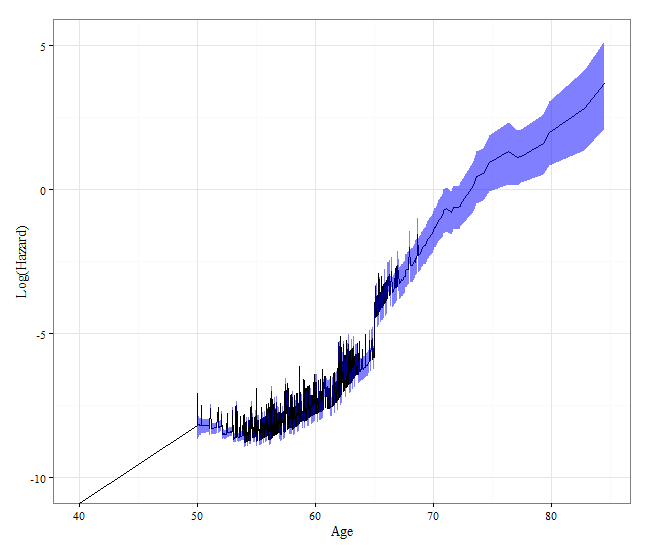
\includegraphics[width=0.35\textwidth]{loghazard.png}}
	\caption{Histogram of Age and point at retire}
	\label{fig:hist}
\end{figure}

%put this graphic in policy discussion part

\subsection{Retirement model without external variables}
Extensive model selection using a variety of metrics including Log likelihood, AIC, BIC,and out of sample predictive scoring (MAPE and $G^2$) was used to identify key predictive factors in the model as shown in table \ref{tab:modelstats}.

% Table generated by Excel2LaTeX from sheet 'summary'
%\begin{landscape}
\begin{table}[htbp]
	\centering
	\scriptsize
	\caption{Models statistics}
	\renewcommand{\arraystretch}{1.5}
	\begin{tabular}{L{3.5cm}lllllrrrr}
		\toprule
	\multicolumn{1}{c}{	\textbf{Model}} & \multicolumn{1}{c}{\textbf{LR}}    & \multicolumn{1}{c}{\textbf{AIC0}}  &\multicolumn{1}{c}{\textbf{AIC}}   &\multicolumn{1}{c}{\textbf{SBC0}} & \multicolumn{1}{c}{\textbf{SBC}}   & \multicolumn{1}{c}{\textbf{\begin{tabular}[c]{@{}c@{}}Pred. \\ MAPE\end{tabular}}} & \multicolumn{1}{c}{\textbf{\begin{tabular}[c]{@{}c@{}}Holdout \\ MAPE\end{tabular}}} &\multicolumn{1}{c}{\textbf{\begin{tabular}[c]{@{}c@{}}Pred. \\ $G^2$\end{tabular}}} & \multicolumn{1}{c}{\textbf{\begin{tabular}[c]{@{}c@{}}Holdout \\ $G^2$\end{tabular}}}  \\
		\midrule
		 Division Gender Payroll Cocs YCSH Ageh & 1194.3 & 20425.6 & 19271.3 & 20425.6 & 19377.3 &  39.44 & 56.78 & 381.77 & 85.19 \\ 
		Division Cocs YCSH Ageh & 1193.77 & 20425.6 & 19269.8 & 20425.6 & 19370.5 &  39.45 & 56.84 & 381.92 & 85.29 \\ 
		Division Policy YCSH Ageh & 1451.62 & 20425.6 & 18998 & 20425.6 & 19061.6 &  25.91 & 15.51 & 128.75 & 2.64 \\ 
		Division Policy YCSH Ageh Cocs & 1469.92 & 20425.6 & 18995.7 & 20425.6 & 19101.7 &   25.91 & 15.24 & 129.47 & 2.56 \\ 
		Division Policy YCSH Ageh and Strata on Cocscode  & 1426.34 & 14602.1 & 13199.8 & 14602.1 & 13263.4 &  43.45 & 87.92 & 186.89 & 50.00 \\ 
		%9 models by Cocscode & N/A   & N/A   & N/A   & N/A   & N/A   &    24.62 & 3.40  & 117.9 & 0.26 \\
		Division Policy YCSH Ageh  P85 & 1826.95 & 20425.6 & 18624.6 & 20425.6 & 18693.6 &  25.59 & 19.04 & 109.17 & 3.40 \\ 
		Division Policy YCSH Ageh  P85 P85*A65 & 1873.69 & 20425.6 & 18579.9 & 20425.6 & 18654.1 &  25.38 & 7.97  & 111.55 & 0.79 \\
		Division Policy YCSH Ageh P85 P85*A65 P85*POLICY & 1881.02 & 20425.6 & 18574.6 & 20425.6 & 18654.1 & 25.42 & 4.20  & 112.27 & 0.81 \\ 
		Logistic regression  & 4103.91 & 13618.4 & 9556.53 & 13627.3 & 9752.1 &  28.20 & 31.73 & 232.84 & 117.38 \\
    	Time series  & N/A   & N/A   & N/A   & N/A   & N/A   &   11.17 & 34.38 & 32.10 & 8.54 \\ 
		\bottomrule
	\end{tabular}%
	\label{tab:modelstats}%
\end{table}%

% Please add the following required packages to your document preamble:

%\end{landscape}

Based on this analysis the optimal modelling variables, excluding aggregate economic factors, chosen for the prediction of age at retirement include {\it division}, {\it years of service at hire}, and {\it age at hire}.  In addition, based on our understanding of the covenants and parameters of the retirement program we tested a number of additional variables and found several that increase the predictive power of the model. These include {\it policy}(an indicator for the 2008 ERI program), {\it P85}(An indicator that the individual has accrued 85 points and can retire with full benefits), {\it A65*P85} (An interaction term that moderates the impact of the {\it P85} effect after the individual has exceeded 65 years of age), and  {\it Policy*P85} (An interaction term that moderates the impact of the {\it P85} effect while the ERI is in place).

Table \ref{tab:paraest.} describes the fit parameters and hazard ratios.  As noted above, we did not find that gender, occupational code and payroll category were not significant predictors in the presence of the other variables. This indicates that employees' gender, job types, and payroll status are not associated with choice of retirement age conditional on the other variables in the model.


% Table generated by Excel2LaTeX from sheet 'Sheet2'
\begin{table}[htbp]
	\centering
	\scriptsize
	\renewcommand{\arraystretch}{1.5}
	\caption{Parameter estimates for models}
	\begin{threeparttable}
	\begin{tabular}{llL{2.5cm}L{1.5cm}L{2.5cm}L{1.5cm}}
		\toprule
		&       & \multicolumn{2}{c}{\textbf{Period Model}} & \multicolumn{2}{c}{\textbf{Yearly model}} \\
		\hline
		Parameter &   Label & Parameter (Standard Error) & Hazard Ratio & Parameter (Standard Error) & Hazard Ratio \\
		\midrule
		    division & dir2  & -0.965(0.179)***\tnote{1} & 0.381 &-1.025(0.177)*** & 0.359 \\
		    division & dir3  & -0.241(0.112)* & 0.786 & -0.246(0.111)* & 0.782 \\
		    division & dir4  & 0.078(0.195) & 1.081 & -0.039(0.195) & 0.962 \\
		    division & dir5  & -0.131(0.190) & 0.877 & -0.246(0.190) & 0.782 \\
		    division & dir6  & 2.136(0.095)*** & 8.463 & 2.252(0.095)*** & 9.511 \\
		    division & dir7  & 2.435(0.129)*** & 11.418 & 2.437(0.129)*** & 11.437 \\
		    division & dir8  & 0.864(0.106)*** & 2.373 & 0.816(0.106)*** & 2.261 \\
		    division & dir9  & -3.023(0.581)*** & 0.049 & -2.774(0.504)*** & 0.062 \\
		    division & dir10 & 0.793(0.093)*** & 2.211 & 0.709(0.093)*** & 2.031 \\
		    YCSH  &       & 0.019(0.004)*** & 1.019 & 0.043(0.004)*** & 1.044 \\
		    Policy & 1     & 0.859(0.169)*** & .     & 0.942(0.109)*** & . \\
		    Ageh &       & -0.172(0.013)*** & 0.842 & -0.187(0.013)*** & 0.829 \\
		    P85   & 1     & 1.435(0.091)*** & .     & 0.682(0.072)*** & . \\
		    A65*P85 & 1     & -1.610(0.206)*** & .     & -0.662(0.177)*** & . \\
		    Policy*P85 & 1     & 0.469(0.179)** & .     & 0.600(0.130)*** & . \\
		\bottomrule
	\end{tabular}%
		\begin{tablenotes}
			\item[1] * denotes $P<0.05$, ** denotes $P<0.01$, and *** denotes $P<0.001$.
		\end{tablenotes}
		
	\end{threeparttable}
	\label{tab:paraest.}%
\end{table}%

{\it P85} is an indicator that a person is eligible for maximum retirement benefits and naturally this has a strong impact on the probability that a person will retire.  From a quantitative point of view the hazard ratio is $e^{1.44} = 4.22$.  So the hazard of retirement becomes 4.22 times more likely after the person exceeds 85 points.  While not surprising, this quantification is important in predicting individual and aggregate retirement time and reflects the modal spike observed in the histogram in Figure \ref{fig:hist}.  The survival function after 85 points is achieved can be su
(Julia, why is the hazard ratio not published in the data??? because it has interaction term)

An alternative eligibility criteria for retirement occurs when individuals exceed an age of 65 years and so we would anticipate the hazard increasing at this point in an employees career.  Because the response variable in our model is age, we cannot estimate the effect of this within the proportional hazards setting because the impact is included in the baseline hazard which should increase after this point; see figure \ref{fig:basepred} (explain).  However, by including an interaction between the indicators of Age greater than 65 and points greater than 85, {\it A65*P85}, we can estimate how the impact of reaching 85 points diminishes when a person exceeds regular retirement age.  In this case, the interaction term is estimated at -1.61 indicating a diminishing effect on the {\it P85} criteria to $e^{1.44-1.61} =0.84$.  This suggests that people that exceed both criteria actually have a reduced hazard of retiring over those have only met the Age 65 criteria.  In other words, the fact that the individual remains on the job after hitting either criteria indicates that the other criteria has less impact (or that they are intending to work longer?).  (Discuss that the baseline may increase so that the overall probability is actually higher.)


According to our model, retirement can also be influenced by an employee's age at hire and their years of service at the time of hiring, {\it YCSH}.  The coefficient estimate for age is -0.17. As the reference age is 45.49, this means that the hazard ratio for retirement of an employee that started working at age 46.49 is $exp(-.017)=.84$ indicating a 16\% drop in hazard for each additional year later that an employee started. The employee's survival probability at any time, $t$, can be computed as $S(t)^{1.19} = (S(t)^{e^{0.17}})$ when age at hire is one year below 45.49,  where $S(t)$ is the baseline survival probability for a reference employee of average age at the time of hiring. Moving in the other direction, employee's survival probability is $S(t)^{0.84}=(S(t)^{e^{-0.17}})$ for a one year increase beyond 45.49 in the employee's starting age. Together, this implies that at any given retirement age, the employee who starts earlier than 45.49 years old is more likely to retire because they have more years of service and closer to vesting full benefits (85 points) than an equivalent employee who starts working at an older age. Similarly, the employee's years of service at hire show a positive estimate (0.019) with a hazard ratio (1.019) indicating that each year of service at hire beyond the baseline of 2.75 is associated with an approximately 2\% increase in the hazard of retirement.  This leads to a survival probability $S(t)^{0.98}$ for a one year decrease in the reference years of service at time of hiring.  On the other hand, the survival probability is $S(t)^{1.019}$ for an employee with one year of service above average at the time of hire. Together, both age at hire and YCSH effects reflect the intuitive fact that, all else being equal, an employee who has more years of service and therefore is closer to full vesting is more likely to retire.  What is non-intuitive about this finding is that while one might suspect that the effects should be of similar magnitude, we actually see that the effect of one year difference in age seems to have about 8 times the impact that one year of previous service does on the hazard of retirement.

\begin{figure}[h!]
	\centering
	\subfloat[Retirement rate]{\label{fig:ratio}\includegraphics[width=0.5\textwidth]{reratio.png}}
	\subfloat[Prediction w/o variable policy]{\label{fig:nopolicy}\includegraphics[width=0.5\textwidth]{nopolicy.png}}
	\caption{Retirement rate and Prediction Plot}
	\label{fig:rerate}
\end{figure}

In the fiscal year 2008, the employer in this study created a temporary early retirement buyout option. The response window for this option was 3 months although the specific details beyond this are unknown. In order to deal with the increased level of retirement during this period we including a time dependent indicator variable.  The coefficient for this indicator was 0.86 leading to a hazard ratio of $e^{.86} = 2.21$ which indicates that, on average, an individuals hazard of retirement increased by almost 2.2 times during this period.  If more information were known about the requirements or targets of this policy, a more case specific estimate may be possible.  However, this would not effect the overall aggregate retirement estimates.  It is important to include this one-time effect in order to improve the estimates of other factors(work on this last part - why do we need to include). 

As a second step, we further test the policy effect on the employees who are eligible for getting a pension. The test results show that the policy had a significant effect for an employee who is eligible for getting the full pension benefit rather than the employee who is only eligible for getting partial retirement as the interaction term of between policy and indicator variables that employees achieve points 75 or points 65 are not statistically significant. The hazard ratio for the policy effect on those employees increases substantially to 15.85 from 2.21, which is more than seven times of the basic policy effect, after the model adding a interaction term of policy and the indicator that a person  exceeds 85 points.


The {\it division} variable was a significant predictor.  For analysis, the baseline level was chosen arbitrarily as division 1 so that it's hazard rate is determined by the baseline.  Relative to this baseline, divisions 6 and 7 have very high hazard ratios, 8.363 and 11.405 respectively, which indicates, other factors being equal, that the employees in division 6 and division 7 are much more likely to retire at any age than those from division 1.  Conversely, division 9 has a hazard ratio of exp(-3.023) = .049 indicating that individuals within this group have 1/20 the hazard of group 1.  This may indicate that the division is new and contains younger employees(how to deal with this??  Time varying variable?).  In general, differences in retirement rates could be caused by differences in age demographics, leadership, departmental and job function, or departmental leadership.

The baseline survival function and log hazard function are shown in figure \ref{fig:basepred}. The survival probability is 1 before age 49 as shown in figure \ref{fig:Surv}, which indicates that no employees retire before this age. The survival probability starts to slowly decease from age 50 to age 62. By age 62 the survival probability has decreased to close to 0.75, which indicates that 75\% of employees retire at an age greater than 62 years.  The slope of survival function decreases sharply at this point indicating the increased retirement rates for workers between age 62 and 65.  After 65 the probability drops off even further as most of the remaining population retires by age 68 or 69. Accompanying the survival function is the log of the cumulative hazard ratio.  Again, the steep rise in the cumulative hazard between age 62 and 65 indicates the increased retirement activity during this period.  After this the cumulative hazard levels off indicating a drop in the hazard rate at these future points.



%Another alternative eligibility criteria occurs when individuals exceed an age of 65 years and so we would anticipate the hazard increasing at this point in an employees career.  Because the response variable in our model is age, we cannot estimate the effect of this within the proportional hazards setting because the impact is included in the baseline hazard which should increase after this point; see figure \ref{fig:basepred} (explain).  However, by including an interaction between the Age 65 and points 85 indicator, we can estimate how the impact of reaching 85 points diminishes beyond regular retirement age.  In this case, the interaction term is estimated at -1.61 leading to a decreasing effect of the 85 points criteria to $e^{1.44-1.61} = 0.84$ indicating that people that exceed both criteria actually have a reduced hazard of retiring over those have only met the Age 65 criteria.  In other words, the fact that the individual remains on the job after hitting either criteria indicates that the other criteria has less impact (or that they are intending to work longer).



%According to our model, retirement can also be influenced by employee's age and their years of service at the time of hiring (YCSH).  The estimates for age are -0.17. As the reference age is 45.49, it means the employee's survival probability is $S(t)^{1.19}(S(t)^{e^{0.17}})$ when the employee started age is one year younger than 45.49,  where $S(t)$ is the baseline survival probability at time t for a reference employee of average age, in the case 45.49 years old at the start of the current interval. The employee's survival probability is $S(t)^{0.84}(S(t)^{e^{-0.17}})$ for every one year increase beyond 45.49 in the employee's starting age. This indicates that at any given age, the employee who starts earlier than 45.49 years old is more likely to retire , because they have more years of service and are much likely to reach retirement requirement (85 points) earlier than the employee who starts at older age. Similar as the years of service, the employee's years of service are hiring time has positive estimates (0.019) with the hazard ratio (1.019). It leads to $S(t)^{0.98}$ of the survival probability for every one year decreasing of the employee in the reference years of service at time of hiring. On the other hand, the survival probability is $S(t)^{1.019}$ for every one year increase of the employee in the reference years of service at hiring time. This indicates that the employee who has more years of service are more likely to retire than the employee who has less years of service.

%In the fiscal year 2008, the employer in the study created a temporary early retirement buyout option. The response window for this option was 3 months although the specific details of this are unknown. In order to deal with the increased level of retirement during this period we including a time dependent indicator variable.  The coefficient for this indicator was 0.86 leading to a hazard ratio of 2.21 which indicates that, on average, an individuals hazard of retirement increased by almost 2.2 times during this period.  If more information were known about the requirements or targets of this policy, a more case specific estimate would be possible.  However, this would not effect the overall aggregate retirement estimates.  It is important to include this one-time effect in order to improve the estimates of other factors(work on this last part - why do we need to include). We further test the policy effect on the employee who are eligible for getting pension. The test results shows the policy had a significant effect for the employee who are eligible for getting the full pension benefit rather than the employee who are eligible for getting partial retirement plan as the interaction term of between policy and points 75 or points 65 are not statistically significant. The hazard ratio for the policy effect on those employee substantially increase to 15.85 from 2.21, which is more than seven times of the basic policy effect, after the model adding a interaction term of policy and points 85.

%Another significant factor is division as shown in the table \ref{tab:paraest.}. As the results shows the employees in some division has positive parameter estimates which is division 6, 7 and 8. Two divisions (division 6 and 7) have very high hazard ratio: 8.46 and 11.42, which indicates that the employee in division 6 and division 7 are much more likely to retire than the employee in reference division (1). Three divisions (2, 3, and 9) have negative estimates (-0.97, -0.24, and -3.02) and the hazard ratios lower than 1 (0.38, 0.79, and 0.05), which indicates the employee in those divisions are much less likely to retire than the employee in reference division (1). Two divisions (4 and 5) are not statistically significant, which indicates that the employee in division 4 and 5 has the similar chance to retire with the employee in the reference division (1). The diversity retirement behavior among divisions might be caused by the diversity of the demographic structure, leadership, departmental function, and departmental culture,

%The baseline survival function and log hazard function are shown in figure \ref{fig:basepred}. The survival probability is 1 before age 49 as shown in figure \ref{fig:Surv}, which indicates that no employee retire before age at 49. Survival probability starts to slowly decease from age 50 to age 62. The survival probability is around 0.75 for the employee who less than 62 years old, which indicates the employee who is less than 62 years has a probability of 25\% to retire.  The slope of survival function decrease sharply and causes the survival probability steeply decreasing from 0.75 to almost 0 from age 62 to age 70, which indicates the employee are much more likely to retire from age 62 to 70. Accompany with the survival function, the log hazard ratio starts to rise up from age 62 and it steps up at age 65 as shown in figure \ref{fig:Hazard}. The trend for hazard function tend to increase by age increasing. The hazard ratio causes the employee retire probability increasing sharply.


Summarize external

Summarize the predictive capabilities at the individual level.  Strengths and weaknesses.

Summarize the predictive capabilities for aggregates.  Strengths and weaknesses.
\begin{figure}[h!]
	\centering
	\subfloat[Survival function]{\label{fig:Surv}\includegraphics[width=0.5\textwidth]{Surv.png}}
	\subfloat[Cumulative hazard]{\label{fig:Cumh}\includegraphics[width=0.5\textwidth]{logcum.png}}
	%\subfloat[Hazard function]{\label{fig:Hazard}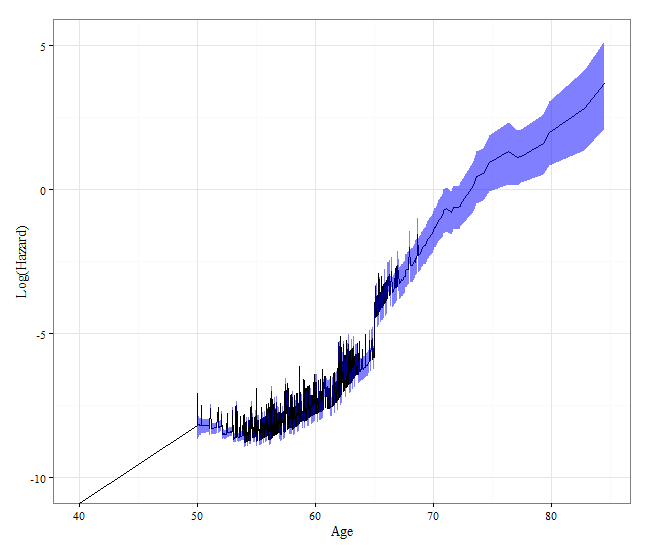
\includegraphics[width=0.35\textwidth]{loghazard.png}}
	\caption{Baselines with 95\% confident intervals}
	\label{fig:basepred}
\end{figure}

{\bf Julia: We need to describe the prediction process results.}

The prediction for the employee retirement is shown in the figure \ref{fig:predict}, table \ref{tab:cocscode} and \ref{tab:division}. The model predictions capture the fluctuations in actual retirement, and also capture the peak of the special year 2008 when an early retirement incentive(policy) was introduced as shown in Figure \ref{fig:predict}. The out of sample predictions for holdout years (2011 and 2012) are very close to the actual number, indicating that the model performs well on both the training and holdout samples. Besides predicting the overall retirement, the model can also provide predictions by category. The table \ref{tab:cocscode} and \ref{tab:division} shows the prediction by occupation code and division by year, which is the summation of the retirement probabilities of individuals by job classification and division, separately. As the tables shown, the predicted values are also close to the actual values in these two categories.

\begin{figure}[h!]
	\centering
	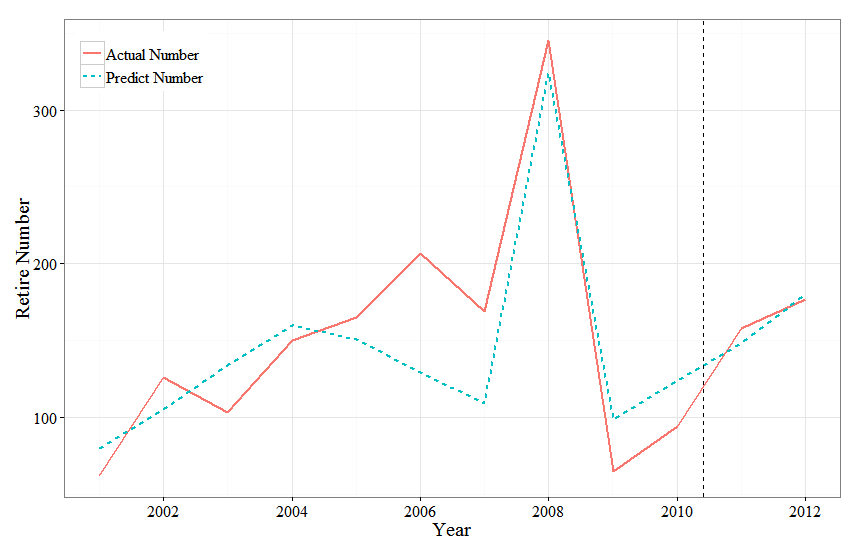
\includegraphics[width=5in]{retire2.png}
	\caption{Retirement Forecasting}
	\label{fig:predict}	
	
\end{figure}

\begin{table}[h!]
	\centering
	\scriptsize
	\smallskip
	\caption{Predictions by job classification}
	\begin{threeparttable}
		\begin{tabular}{cL{1.2cm}L{1.2cm}L{1.2cm}L{1.2cm}L{1.2cm}L{1.2cm}L{1.2cm}L{1.2cm}L{1.2cm}l}
			\toprule
			Year  &  Crafts & Engineers& General Admin. & Laborers& Managers& Prof. Admin.& Operators& Scientists& Technicians& Total \\
			\midrule
%			2001  & 23\tnote{1} (16)\tnote{2} & 12 (10) & 4 (1) & 6 (5) & 11 (14) & 10 (9) & 8 (2) & 2 (1) & 4 (4) & 80 (62) \\
%			2002  & 31 (29) & 15 (16) & 5 (15) & 7 (11) & 15 (26) & 13 (18) & 11 (6) & 2 (1) & 6 (4) & 105 (126) \\
%			2003  & 37 (26) & 19 (13) & 6 (5) & 9 (6) & 17 (21) & 18 (13) & 16 (15) & 4 (2) & 8 (2) & 134 (103) \\
%			2004  & 44 (32) & 23 (23) & 8 (9) & 11 (7) & 21 (30) & 23 (25) & 16 (15) & 4 (3) & 10 (6) & 160 (150) \\
%			2005  & 40 (39) & 24 (17) & 8 (13) & 9 (7) & 20 (27) & 24 (31) & 12 (15) & 3 (4) & 11 (12) & 151 (165) \\
%			2006  & 31 (58) & 20 (29) & 6 (10) & 8 (9) & 19 (32) & 25 (37) & 9 (13) & 2 (4) & 9 (15) & 129 (207) \\
%			2007  & 19 (44) & 14 (25) & 7 (9) & 6 (9) & 18 (26) & 27 (40) & 8 (6) & 3 (4) & 7 (6) & 109 (169) \\
%			2008  & 54 (71) & 30 (33) & 20 (20) & 22 (12) & 64 (63) & 80 (84) & 26 (32) & 6 (7) & 22 (23) & 324 (345) \\
%			2009  & 16 (14) & 9 (6) & 7 (3) & 7 (7) & 21 (8) & 25 (10) & 8 (11) & 1 (1) & 5 (5) & 99 (65) \\
%			2010  & 19 (19) & 11 (17) & 9 (1) & 7 (8) & 28 (23) & 34 (16) & 8 (4) & 1 (3) & 7 (3) & 124 (94) \\
%			2011  & 22 (36) & 13 (25) & 11 (8) & 9 (9) & 34 (27) & 40 (34) & 9 (5) & 2 (1) & 8 (13) & 148 (158) \\
%			2012  & 24 (29) & 16 (23) & 14 (11) & 12 (10) & 41 (46) & 49 (36) & 12 (4) & 3 (2) & 9 (16) & 180 (177) \\
    2001  & 23\tnote{1} (16)\tnote{2} & 12 (10) & 4 (1) & 6 (5) & 11 (14) & 11 (9) & 8 (2) & 2 (1) & 4 (4) & 81 (62) \\
    2002  & 31 (29) & 15 (16) & 5 (15) & 7 (11) & 15 (26) & 13 (18) & 11 (6) & 2 (1) & 6 (4) & 105 (126) \\
    2003  & 37 (26) & 18 (13) & 6 (5) & 9 (6) & 17 (21) & 18 (13) & 16 (15) & 4 (2) & 8 (2) & 133 (103) \\
    2004  & 43 (32) & 23 (23) & 8 (9) & 11 (7) & 21 (30) & 23 (25) & 15 (15) & 4 (3) & 10 (6) & 158 (150) \\
    2005  & 40 (39) & 24 (17) & 8 (13) & 9 (7) & 20 (27) & 24 (31) & 12 (15) & 3 (4) & 11 (12) & 151 (165) \\
    2006  & 31 (58) & 20 (29) & 6 (10) & 8 (9) & 19 (32) & 25 (37) & 9 (13) & 2 (4) & 9 (15) & 129 (207) \\
    2007  & 19 (44) & 14 (25) & 7 (9) & 6 (9) & 18 (26) & 27 (40) & 8 (6) & 3 (4) & 7 (6) & 109 (169) \\
    2008  & 55 (71) & 30 (33) & 19 (20) & 22 (12) & 64 (63) & 79 (84) & 27 (32) & 6 (7) & 21 (23) & 323 (345) \\
    2009  & 16 (14) & 9 (6) & 7 (3) & 7 (7) & 20 (8) & 25 (10) & 8 (11) & 1 (1) & 5 (5) & 98 (65) \\
    2010  & 18 (19) & 11 (17) & 9 (1) & 7 (8) & 28 (23) & 34 (16) & 8 (4) & 1 (3) & 7 (3) & 123 (94) \\
    2011  & 22 (36) & 13 (25) & 11 (8) & 9 (9) & 34 (27) & 40 (34) & 9 (5) & 2 (1) & 8 (13) & 148 (158) \\
    2012  & 24 (29) & 16 (23) & 14 (11) & 12 (10) & 41 (46) & 49 (36) & 12 (4) & 3 (2) & 9 (16) & 180 (177) \\

			\bottomrule
		\end{tabular}%
		\begin{tablenotes}
			\item[1] the number before the parentheses is predicted retirement number.
			\item[2] the number inside the parentheses is actual retirement number.
		\end{tablenotes}
		
	\end{threeparttable}
	\label{tab:cocscode}
\end{table}


% Table generated by Excel2LaTeX from sheet 'Sheet4'
\begin{table}[h!]
	\centering
	\scriptsize
	\caption{Prediction by division}
	\begin{threeparttable}
		\begin{tabular}{clllllllllll}
			\toprule
			Year  & \multicolumn{1}{c}{Division1} & \multicolumn{1}{c}{Division2} & \multicolumn{1}{c}{Division3} & \multicolumn{1}{c}{Division4} & \multicolumn{1}{c}{Division5} & \multicolumn{1}{c}{Division6} & \multicolumn{1}{c}{Division7} & \multicolumn{1}{c}{Division8} & \multicolumn{1}{c}{Division9} & \multicolumn{1}{c}{Division10} \\
			\midrule
%			2001  & 3\tnote{1} (0)\tnote{2} & 0 (0) & 1 (0) & 0 (0) & 0 (0) & 56 (43) & 11 (2) & 5 (10) & 0 (0) & 5 (7) \\
%			2002  & 4 (0) & 0 (0) & 2 (0) & 0 (0) & 0 (0) & 72 (54) & 14 (2) & 6 (38) & 0 (0) & 8 (32) \\
%			2003  & 6 (0) & 1 (0) & 2 (0) & 0 (0) & 0 (0) & 89 (44) & 19 (7) & 6 (18) & 0 (0) & 9 (34) \\
%			2004  & 9 (0) & 1 (0) & 4 (0) & 1 (0) & 1 (0) & 101 (96) & 26 (29) & 7 (13) & 0 (0) & 10 (12) \\
%			2005  & 13 (0) & 1 (0) & 5 (0) & 1 (0) & 1 (0) & 88 (114) & 20 (26) & 8 (18) & 0 (0) & 14 (7) \\
%			2006  & 19 (34) & 2 (0) & 8 (0) & 2 (5) & 2 (3) & 58 (105) & 12 (32) & 9 (12) & 0 (0) & 17 (16) \\
%			2007  & 23 (59) & 3 (0) & 12 (5) & 3 (7) & 3 (9) & 26 (53) & 3 (10) & 12 (6) & 0 (0) & 24 (20) \\
%			2008  & 85 (97) & 14 (23) & 51 (79) & 11 (11) & 12 (13) & 16 (16) & 0 (0) & 45 (24) & 1 (0) & 86 (82) \\
%			2009  & 27 (17) & 5 (4) & 15 (21) & 4 (3) & 4 (3) & 0 (0) & 0 (0) & 16 (4) & 0 (0) & 27 (13) \\
%			2010  & 32 (25) & 7 (10) & 19 (20) & 6 (4) & 6 (4) & 0 (0) & 0 (0) & 23 (6) & 1 (4) & 32 (21) \\
%			2011  & 38 (51) & 9 (15) & 23 (25) & 7 (8) & 7 (9) & 0 (0) & 0 (0) & 28 (12) & 1 (15) & 34 (23) \\
%			2012  & 42 (36) & 13 (15) & 30 (15) & 9 (3) & 10 (3) & 0 (0) & 0 (0) & 32 (14) & 1 (8) & 41 (15) \\
        2001  & 3\tnote{1} (0)\tnote{2} & 0 (0) & 1 (0) & 0 (0) & 0 (0) & 57 (43) & 11 (2) & 5 (10) & 0 (0) & 5 (7) \\
        2002  & 4 (0) & 0 (0) & 2 (0) & 0 (0) & 0 (0) & 72 (54) & 14 (2) & 6 (38) & 0 (0) & 9 (32) \\
        2003  & 6 (0) & 1 (0) & 2 (0) & 1 (0) & 0 (0) & 89 (44) & 19 (7) & 6 (18) & 0 (0) & 9 (34) \\
        2004  & 9 (0) & 1 (0) & 4 (0) & 1 (0) & 1 (0) & 101 (96) & 26 (29) & 7 (13) & 0 (0) & 10 (12) \\
        2005  & 13 (0) & 1 (0) & 5 (0) & 1 (0) & 1 (0) & 87 (114) & 20 (26) & 8 (18) & 0 (0) & 14 (7) \\
        2006  & 18 (34) & 2 (0) & 8 (0) & 2 (5) & 2 (3) & 58 (105) & 12 (32) & 9 (12) & 0 (0) & 17 (16) \\
        2007  & 23 (59) & 3 (0) & 12 (5) & 3 (7) & 3 (9) & 26 (53) & 3 (10) & 12 (6) & 0 (0) & 24 (20) \\
        2008  & 87 (97) & 14 (23) & 52 (79) & 11 (11) & 12 (13) & 16 (16) & 0 (0) & 45 (24) & 1 (0) & 85 (82) \\
        2009  & 26 (17) & 5 (4) & 15 (21) & 4 (3) & 5 (3) & 0 (0) & 0 (0) & 16 (4) & 0 (0) & 27 (13) \\
        2010  & 32 (25) & 7 (10) & 18 (20) & 6 (4) & 6 (4) & 0 (0) & 0 (0) & 23 (6) & 1 (4) & 32 (21) \\
        2011  & 38 (51) & 9 (15) & 23 (25) & 7 (8) & 7 (9) & 0 (0) & 0 (0) & 28 (12) & 1 (15) & 35 (23) \\
        2012  & 42 (44) & 13 (16) & 30 (33) & 9 (3) & 10 (7) & 0 (0) & 0 (0) & 32 (21) & 1 (15) & 42 (38) \\
              

			\bottomrule
		\end{tabular}%
		\begin{tablenotes}
			\item[1] the number before the parentheses is predicted retirement number.
			\item[2] the number inside the parentheses is actual retirement number.
		\end{tablenotes}
	\end{threeparttable}
	\label{tab:division}%
\end{table}%


%\item Employee Profile 1: The employee's pattern for employees retire right away.

%\item Employee Profile 2: The employee's pattern who did not retire after eligible for retirement.

%\item New Chapter: Short term prediction model.  Logistic regression for 1 year on elgible retirees.  Possible prediction?




\subsection{Retirement model with external variables}
  Because the previous model cannot account for the time varying features of the economic indicators, we use a new counting process model with yearly interval based on calendar year to test their effects on retirement. This model has the similar parameter estimation as the selected model as shown in the right part of the table \ref{tab:paraest.}. We found three indicators are statistically significant and also improve the model forecasting due to lower MAPE and $G^2$ than the values of selected model without economic indicator, which are S\&P500, Real Earnings and Wilshire 5000 as shown in table \ref{tab:EI}. Although Real price is also statistically significant, its coefficient estimates is 0.0004 leading hazard ratio is 1, which indicate it does not impact the employee's retirement behaviors. As shown in table \ref{tab:EI}, Real earnings is the most important factor among all the indicators as it has lowest $G^2$. The test results show that it has strong impact on the retire behaviors. As shown in figure \ref{fig:real}, the fluctuation of retirement plot is corresponding with 1 year lag of the trend of Real earnings. Unadjusted Monthly Housing Price (MHP) is another influential index with the lowest MAPE value. It has significantly impacts on the retire number as it increases as shown in figure \ref{fig:MHP}. However, the retire number does not decrease coinciding with the decreasing of MHP. Two market indicators(S\&P500 and Wilshire 5000) are both significantly impact the employee retirement behavior with $>1$ hazard ratio, which indicating the employee are more likely to retire when the economics is under good condition. 
\begin{table}[htbp]
	\scriptsize
	\centering
	\caption{Economic index test statistics}
	\begin{threeparttable}
	\begin{tabular}{L{3cm}ccccc}
		\toprule
		\textbf{Economic Inidcator} &\multicolumn{1}{c}{\textbf{$\chi^2$}} &  \multicolumn{1}{c}{\textbf{P-value}} & \multicolumn{1}{c}{\textbf{\begin{tabular}[c]{@{}c@{}}Hazard \\ ratio\end{tabular}}}   &  \multicolumn{1}{c}{\textbf{MAPE}} &\multicolumn{1}{c}{\textbf{$G^2$}} \\
		\midrule
	Without Econmic indicator\tnote{1} &       &       &       & 21.31 & 147.43 \\
	MHP NSA & 129.614 & $<.001$ & 1.020  & 17.84 & 220.65 \\
	MHP SA & 129.516 & $<.001$ & 1.020  & 17.86 & 221.66 \\
	Southeast MHP NSA & 68.055 & $<.001$ & 1.030  & 23.37 & 178.38 \\
	Southeast MHP SA & 67.871 & $<.001$& 1.030  & 23.40 & 179.87 \\
	S\&P500 & 13.319 & $<.001$ & 1.001 & 20.79 & 129.83 \\
	Dividend & 1.045 & 0.307 & 1.015 & 22.63 & 150.03 \\
	Earnings & 84.895 & $<.001$ & 1.016 & 21.40 & 105.06 \\
	Consumer Price Index & 5.404 & 0.020 & 1.013 & 21.36 & 133.57 \\
	Real Price & 5.522 & 0.019 & 1.000     & 21.22 & 138.72 \\
	Real Dividend & 1.925 & 0.165 & 1.022 & 23.39 & 154.84 \\
	Real Earnings & 80.358 & $<.001$ & 1.013 & 20.33 & 95.02 \\
	Long Interest Rate & 1.539 & 0.215 & 1.082 & 22.03 & 149.01 \\
	Unemployment Rate & 32.212 & $<.001$ & 0.849 & 25.08 & 179.49 \\
	P E10 & 0.041 & 0.839 & 0.998 & 21.31 & 147.97 \\
	Wilshire5000 & 22.392 & $<.001$ & 1.028 & 20.83 & 121.58 \\
		\bottomrule
	\end{tabular}%
	\begin{tablenotes}
		\item[1] it is the selected model without economic indicator.
	\end{tablenotes}
\end{threeparttable}
	\label{tab:EI}%
\end{table}%
\begin{figure}[h!]
	\centering
	\subfloat[Monthly Housing Price]{\label{fig:MHP}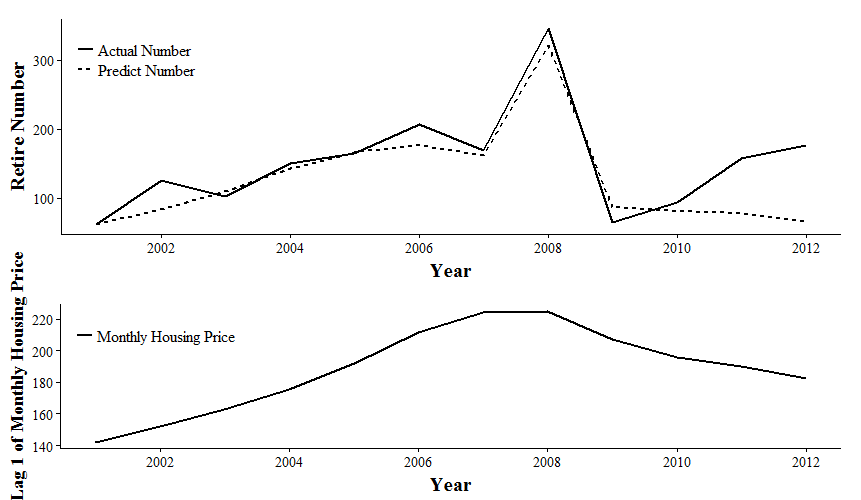
\includegraphics[width=0.5\textwidth]{MHP.png}}
	\subfloat[Real Earnings]{\label{fig:Real}\includegraphics[width=0.5\textwidth]{realearnings.png}}
	%\subfloat[Hazard function]{\label{fig:Hazard}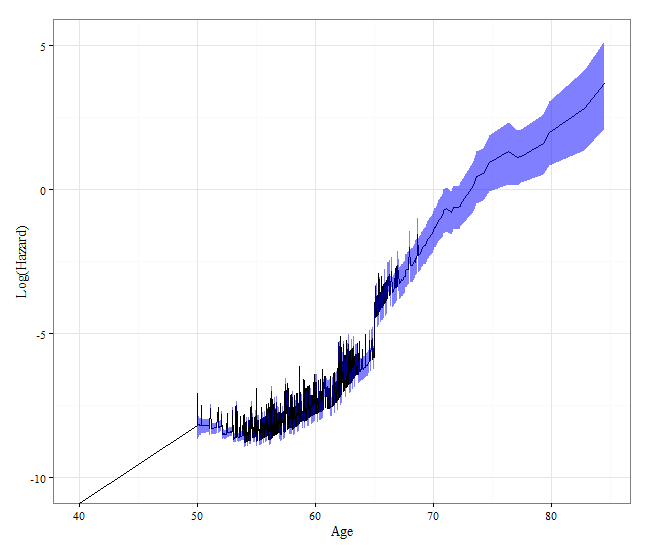
\includegraphics[width=0.35\textwidth]{loghazard.png}}
	\caption{Economic indicators and retirement prediciting plot}
	\label{fig:EIndex}
\end{figure}

\subsubsection{Voluntary quit model without external variables}   
I. dependent variable are YCSH, because age is not able to predict well. Why plot YCSH by vq and age by vq to discribe why.
one employee quit with 67 years old and less than 85 points. all quit before 65 years.
II. shorten the length of risk set. how to shorten the risk set. 
iii. model comparison. (survival model, time seris model, and logsitic regression model)
\subsubsection{Voluntary quit model with external variables}
i. tested which variable does significantly impact on employee voluntary quit.

\section{Conclusions and Managerial Implications}
Conclusions and Managerial Implications

1) We were construct an individual level retirement model for current and past workers that accurately predicted yearly retirement levels.

2) A semi-parametric cox proportional hazards model was used to model age at retirement.  The model investigated demographic, organizational, and macroeconomic factors that might impact the retirement decision.

3) Factors that had the strongest influence included years of service, whether or not an ERP was in effect, whether or not the individual exceeded the number of points required for full retirement benefits.  The most valuable external factor impacting retirement decisions is the Real Earnings as defined by the bureau of labor statistics.

4) Discuss impacts captured by baseline.

5) Factors that did not seem to significantly impact retirement decisions included gender, payroll classification, job classification code, and a large number of additional macroeconomic indicators.

6) The model was tested and was able to accurately predict number of retirements up to two years into the future.  It may be accurate beyond that as well but sufficient data was not available to test this.

7) Why might real earnings be important.

8) Moderating effect of age.  Workers that stayed beyond the term required for full benefits were seen to have much reduced probabilities of retiring as indicated by a moderating interaction indicator.


Managerial Implications....

	\bibliographystyle{abbrvnat}%Choose a bibliograhpic style%
	\bibliography{Bib}
\end{document}
